% =============================================================
% BÖLÜM 4: RISC-V ile Programlama
% Bilgisayar Mimarisi Kitabı
% Oğuz Ergin
% =============================================================

\chapter{RISC-V ile Programlama}
\label{chap:programlama}
\bolumfoto[Hititler, 3700 yıl önce kil tabletlere çivi yazısıyla buyruklar kazıdı. Bugün programcılar da benzer bir iş yapar: buyruğu satır satır yazarak bilgisayara ne yapacağını anlatır.]{gorseller/bolum04-hattusa.jpg}{Hattuşa Aslan Kapısı -- Çorum}

\begin{tcolorbox}[
    colframe=sinyalyesil!60!black,
    title={\textbf{Öğrenme Hedefleri}},
    fonttitle=\bfseries,
    rounded corners,
    boxrule=0.8pt
]
Bu bölümü tamamladığınızda aşağıdakileri yapabileceksiniz:
\begin{itemize}[nosep, leftmargin=*]
    \item RISC-V çevirici dilinde baştan sona çalışan programlar yazmak.
    \item Dizi, karakter dizisi ve yapı gibi veri yapılarını bellekte düzenleyip işlemek.
    \item C dilinde yazılmış bir programın RISC-V çevirici diline nasıl derlendiğini okuyup yorumlamak.
    \item Derleyicinin farklı eniyileme seviyelerinde ürettiği kodu karşılaştırmak.
    \item Bellek eşlemeli giriş/çıkış ile basit bir gömülü sistem programı yazmak.
    \item Döngü ve bellek erişim kalıplarını başarım açısından değerlendirmek.
    \item Çevirici dil programlarında hata ayıklama yapmak.
\end{itemize}
\end{tcolorbox}

\section*{Giriş}

Bir önceki bölümde RISC-V buyruk kümesini öğrendik: yazmaçları, aritmetik ve mantık buyruklarını, bellek erişim buyruklarını, dallanma ve atlama buyruklarını, fonksiyon çağrılarını ve yığıt yönetimini gördük. Ancak bu buyrukları tek tek tanımak, bunlarla gerçek bir program yazabilmek için yeterli değildir. Tıpkı bir dilin sözcüklerini bilmenin o dilde roman yazmaya yetmemesi gibi, buyrukları bilmek de programlamaya yetmez; sözcüklerden cümle kurmayı, cümlelerden paragraf oluşturmayı öğrenmek gerekir.

Bu bölümde, önceki bölümde öğrendiğimiz buyrukları kullanarak baştan sona çalışan programlar yazacağız. Amacımız yalnızca çevirici dil öğretmek değil, aynı zamanda bilgisayar mimarisini ``içeriden'' anlamaktır: bir C programının makine düzeyinde nasıl çalıştığını görmek, derleyicinin hangi kararları neden aldığını kavramak ve donanımın yazılımla nasıl etkileştiğini gözlemlemek. Bu bakış açısı, ileriki bölümlerde işlemci tasarımı, boru hattı ve bellek hiyerarşisi konularına geçtiğimizde güçlü bir temel oluşturacaktır.

Bölümün akışı kademeli bir zorluk sırası izler: önce en basit yazmaç ve bellek işlemleriyle başlayacağız, sonra program yapısını ve geliştirme ortamını tanıyacağız, ardından algoritmalar ve veri yapılarına geçeceğiz.


% =====================================================
\section{İlk Adımlar}
\label{sec:ilk-adimlar}
\index{RISC-V!ilk adımlar}

Çevirici dil programlamaya en basit işlemle başlayalım: iki sayıyı toplamak. Aşağıdaki örnekler RARS benzeticisinde çalıştırılmak üzere tasarlanmıştır; her birini yazıp çalıştırmanız ve yazmaç değerlerini gözlemlemeniz önerilir. Her örnekte bir başarım çözümlemesi de yapacağız; böylece Bölüm~\ref{chap:basarim}'de öğrendiğimiz kavramları uygulamaya koymuş olacağız.

\subsection{Yazmaçlarla Aritmetik}
\label{subsec:yazmaclarla-aritmetik}

\begin{ornek}[4.1]
\label{orn:iki-yazmac-topla}
İki yazmaca sabit değerler yükleyip bunları toplayın. Sonucu ekrana yazdırın.

\textbf{Çözüm:}

\begin{lstlisting}[style=riscv]
.text
.globl main
main:
    li   t0, 25               # t0 = 25
    li   t1, 17               # t1 = 17
    add  t2, t0, t1           # t2 = t0 + t1 = 42

    # Sonucu ekrana yazdır
    mv   a0, t2               # a0 = yazdırılacak değer
    li   a7, 1                # 1 = tam sayı yazdır
    ecall

    # Programı sonlandır
    li   a7, 10
    ecall
\end{lstlisting}

Programın son dört satırında kullanılan \texttt{ecall} (\emph{environment call}) buyruğu, programın işletim sisteminden bir hizmet istemesini sağlar; tıpkı bir restoranda müşterinin garsona sipariş vermesi gibi. Hangi hizmetin isteneceği \texttt{a7} yazmacına yazılan numarayla belirlenir: \texttt{a7\,=\,1} ``\texttt{a0}'daki tam sayıyı ekrana yaz'' demektir; \texttt{a7\,=\,10} ise ``programı sonlandır'' anlamına gelir. İşletim sistemi bu numaraya bakarak doğru hizmeti çalıştırır; bu mekanizmaya \emph{sistem çağrısı} (\emph{system call}) denir ve Bölüm~\ref{chap:giris-cikis}'da ayrıntılı olarak ele alınacaktır.

Bu programdaki \texttt{li} ve \texttt{mv} buyrukları aslında sözde buyruktur (\emph{pseudo-instruction}); çevirici bunları gerçek RISC-V buyrukları ile değiştirir (Bölüm~\ref{chap:buyruk-kumesi}'teki Tablo~\ref{tab:sozde-buyruklar}'ı hatırlayın). Aşağıdaki tablo bu dönüşümü somut bir program üzerinde gösterir:

\begin{center}
\small
\begin{tabular}{lll}
\toprule
\texttt{Sözde buyruk} & \texttt{Gerçek buyruk} & Açıklama \\
\midrule
\texttt{li t0, 25}  & \texttt{addi t0, x0, 25} & \texttt{x0} her zaman 0'dır \\
\texttt{li t1, 17}  & \texttt{addi t1, x0, 17} & $0 + 17 = 17$ \\
\texttt{add t2, t0, t1} & \texttt{add t2, t0, t1} & Zaten gerçek buyruk \\
\texttt{mv a0, t2}  & \texttt{addi a0, t2, 0}  & $\texttt{t2} + 0 = \texttt{t2}$ \\
\texttt{li a7, 1}   & \texttt{addi a7, x0, 1}  & Sistem çağrısı numarası \\
\texttt{ecall}       & \texttt{ecall}            & Zaten gerçek buyruk \\
\texttt{li a7, 10}  & \texttt{addi a7, x0, 10} & Program sonlandırma \\
\texttt{ecall}       & \texttt{ecall}            & Zaten gerçek buyruk \\
\bottomrule
\end{tabular}

Buyruk adlarının açılımları: \texttt{li} = \emph{load immediate} (anlık değer yükle), \texttt{add} = \emph{add} (topla), \texttt{addi} = \emph{add immediate} (anlık değerle topla), \texttt{mv} = \emph{move} (taşı), \texttt{ecall} = \emph{environment call} (ortam çağrısı).
\end{center}

İşlemcinin gerçekte yürüttüğü buyruklar sağ sütundakilerdir. RARS'ta ``Execute'' sekmesinde ``Basic'' sütununa bakarsanız bu dönüşümü görebilirsiniz. Şimdi her buyruğun yazmaçları nasıl değiştirdiğini izleyelim:

\begin{center}
\small
\begin{tabular}{clccccc}
\toprule
\texttt{\#} & Gerçek buyruk & \texttt{t0} & \texttt{t1} & \texttt{t2} & \texttt{a0} & \texttt{a7} \\
\midrule
  & \emph{(başlangıç)} & 0 & 0 & 0 & 0 & 0 \\
1 & \texttt{addi t0, x0, 25} & \underline{25} & 0 & 0 & 0 & 0 \\
2 & \texttt{addi t1, x0, 17} & 25 & \underline{17} & 0 & 0 & 0 \\
3 & \texttt{add t2, t0, t1}  & 25 & 17 & \underline{42} & 0 & 0 \\
4 & \texttt{addi a0, t2, 0}  & 25 & 17 & 42 & \underline{42} & 0 \\
5 & \texttt{addi a7, x0, 1}  & 25 & 17 & 42 & 42 & \underline{1} \\
6 & \texttt{ecall}            & 25 & 17 & 42 & 42 & 1 \\
7 & \texttt{addi a7, x0, 10} & 25 & 17 & 42 & 42 & \underline{10} \\
8 & \texttt{ecall}            & 25 & 17 & 42 & 42 & 10 \\
\bottomrule
\end{tabular}
\end{center}

Altı çizili değerler o adımda değişen yazmaçlardır. Tablodan görüldüğü gibi her buyruk yalnızca \emph{tek bir} hedef yazmacı değiştirir; bu, RISC mimarilerinin temel özelliğidir.

\emph{Başarım çözümlemesi:} Program 8 gerçek buyruktan oluşur. Tümü yazmaç işlemi veya sistem çağrısıdır; bellek erişimi yoktur. Her buyruk tek çevrimde tamamlansa toplam $8 \times 1 = 8$ çevrimdir ve BBÇ~$= 1{,}0$ olur. Bu, bir programın ulaşabileceği en iyi BBÇ değeridir: bellek erişimi olmayan, dallanma içermeyen düz bir kod akışı.
\end{ornek}

\subsection{Bellekten Okuma ve Yazma}
\label{subsec:bellekten-okuma-yazma}

\begin{ornek}[4.2]
\label{orn:bellek-oku-yaz}
Bellekteki bir değeri yazmaca yükleyin, üzerine bir sayı ekleyin ve sonucu belleğe geri yazın.

\textbf{Çözüm:}

\begin{lstlisting}[style=riscv]
.data
sayi:    .word  100           # bellekte saklanan değer
sonuc:   .word  0             # sonuç buraya yazılacak

.text
.globl main
main:
    la   t0, sayi             # t0 = sayi'nın adresi
    lw   t1, 0(t0)           # t1 = bellekteki değer (100)
    addi t1, t1, 50          # t1 = 100 + 50 = 150

    la   t2, sonuc            # t2 = sonuc'un adresi
    sw   t1, 0(t2)           # sonucu belleğe yaz

    # Sonucu ekrana yazdır
    mv   a0, t1              # yazdırılacak değer
    li   a7, 1               # 1 = tam sayı yazdır
    ecall

    li   a7, 10              # 10 = programı sonlandır
    ecall
\end{lstlisting}

Bu örnekte dört yeni buyruk kullanılmaktadır: \texttt{la} (\emph{load address}, adres yükle) bir verinin bellekteki adresini yazmaca yükler; \texttt{lw} (\emph{load word}, sözcük yükle) o adresteki 4 baytlık değeri yazmaca okur; \texttt{sw} (\emph{store word}, sözcük sakla) yazmaçtaki değeri belleğe yazar; \texttt{auipc} (\emph{add upper immediate to PC}, üst anlık değeri program sayacına ekle) ise \texttt{la}'nın gerçek buyruk karşılığının ilk yarısıdır. Sözde buyruk dönüşümüne bakalım; burada önemli bir fark vardır:

\begin{center}
\small
\begin{tabular}{lll}
\toprule
\texttt{Sözde buyruk} & \texttt{Gerçek buyruk(lar)} & Açıklama \\
\midrule
\multirow{2}{*}{\texttt{la t0, sayi}} & \texttt{auipc t0, \%hi(sayi)} & Üst 20 bit: PC + üst adres \\
                                       & \texttt{addi t0, t0, \%lo(sayi)} & Alt 12 bit: tam adres \\
\texttt{lw t1, 0(t0)} & \texttt{lw t1, 0(t0)} & Zaten gerçek buyruk \\
\texttt{addi t1, t1, 50} & \texttt{addi t1, t1, 50} & Zaten gerçek buyruk \\
\multirow{2}{*}{\texttt{la t2, sonuc}} & \texttt{auipc t2, \%hi(sonuc)} & Üst 20 bit \\
                                        & \texttt{addi t2, t2, \%lo(sonuc)} & Alt 12 bit \\
\texttt{sw t1, 0(t2)} & \texttt{sw t1, 0(t2)} & Zaten gerçek buyruk \\
\texttt{mv a0, t1}  & \texttt{addi a0, t1, 0}  & $\texttt{t1} + 0$ \\
\texttt{li a7, 1}   & \texttt{addi a7, x0, 1}  & Sistem çağrısı \\
\texttt{ecall}       & \texttt{ecall}            & --- \\
\texttt{li a7, 10}  & \texttt{addi a7, x0, 10} & Program sonu \\
\texttt{ecall}       & \texttt{ecall}            & --- \\
\bottomrule
\end{tabular}
\end{center}

Dikkat: \texttt{la} sözde buyruğu \emph{iki} gerçek buyruğa açılır çünkü 32 bitlik bir adres tek buyruğun 12 bitlik sabit alanına sığmaz. \texttt{auipc} üst 20 biti, \texttt{addi} alt 12 biti birleştirerek tam adresi oluşturur. Bu nedenle programdaki 10 sözde buyruk aslında 12 gerçek buyruğa dönüşür. Bu durum, Bölüm~\ref{chap:basarim}'de tanıttığımız üç farklı buyruk sayısını somut biçimde örnekler:

\begin{center}
\small
\begin{tabular}{lcc}
\toprule
Buyruk türü & Sayı & Belirleyen \\
\midrule
Programcının yazdığı (sözde buyruklar dahil) & 10 & Programcı \\
Durağan (bellekteki gerçek buyruklar) & 12 & Çevirici \\
Devingen (yürütülen toplam buyruk) & 12 & İşlemci \\
\bottomrule
\end{tabular}
\end{center}

Bu programda döngü olmadığı için durağan ve devingen sayı birbirine eşittir. Ancak başarım hesaplamalarında her zaman durağan veya devingen buyruk sayısını kullanmalıyız; programcının yazdığı sözde buyruk sayısını değil.

Yazmaç ve bellek değişim tablosu (\texttt{sayi} adresi \texttt{0x10000000}, \texttt{sonuc} adresi \texttt{0x10000004} varsayılmıştır):

\begin{center}
\small
\begin{tabular}{clccccc}
\toprule
\texttt{\#} & Gerçek buyruk & \texttt{t0} & \texttt{t1} & \texttt{t2} & \texttt{a0} & Bellek \\
\midrule
   & \emph{(başlangıç)} & 0 & 0 & 0 & 0 & \texttt{[sayi]=100, [sonuc]=0} \\
1--2 & \texttt{auipc+addi} (la t0, sayi) & \underline{0x...0000} & 0 & 0 & 0 & --- \\
3 & \texttt{lw t1, 0(t0)} & 0x...0000 & \underline{100} & 0 & 0 & \emph{okuma} \\
4 & \texttt{addi t1, t1, 50} & 0x...0000 & \underline{150} & 0 & 0 & --- \\
5--6 & \texttt{auipc+addi} (la t2, sonuc) & 0x...0000 & 150 & \underline{0x...0004} & 0 & --- \\
7 & \texttt{sw t1, 0(t2)} & 0x...0000 & 150 & 0x...0004 & 0 & \underline{\texttt{[sonuc]=150}} \\
8 & \texttt{addi a0, t1, 0} & 0x...0000 & 150 & 0x...0004 & \underline{150} & --- \\
\bottomrule
\end{tabular}
\end{center}

Bu tabloda Örnek~4.1'den farklı olarak ``Bellek'' sütunu eklendi. 3.~adımda bellekten okuma, 7.~adımda belleğe yazma yapılır. RARS'ta ``Data Segment'' sekmesini izleyerek bu değişimleri doğrulayın.

\emph{Başarım çözümlemesi:} İşlemci 12 gerçek buyruk yürütür (sözde buyruk sayısı 10 olsa da). Bunların 2'si bellek erişimi (\texttt{lw}, \texttt{sw}), 10'u yazmaç işlemidir. Yazmaç buyrukları 1, bellek buyrukları 2 çevrimle: $10 \times 1 + 2 \times 2 = 14$ çevrim, BBÇ~$= 14/12 \approx 1{,}17$. Sözde buyrukların gerçek buyruk sayısını artırabileceğine dikkat edin: buyruk sayarken her zaman gerçek buyrukları saymalıyız. Bellek erişim gecikmelerinin önbellek hiyerarşisiyle nasıl azaltıldığını Bölüm~\ref{chap:bellek}'de ayrıntılı olarak ele alacağız.
\end{ornek}

\begin{bilginot}[\texttt{auipc} ve Program Sayacı]
\texttt{auipc} (\emph{add upper immediate to PC}) buyruğu, 20 bitlik sabiti 12 bit sola kaydırıp \emph{o anki PS değerine} ekler. Burada kritik nokta şudur: PS, \texttt{auipc} buyruğunun kendisinin bellekteki adresini gösterir, bir sonraki buyruğun adresini değil. Bu sayede \texttt{auipc} + \texttt{addi} çifti, buyruğun bellekteki konumundan bağımsız olarak hedef adrese ulaşabilir (\emph{konumdan bağımsız kod}, \emph{position-independent code}).

Örnek: \texttt{auipc t0, 0x12345} buyruğu \texttt{0x0000\_2000} adresindeyse:
\[
\texttt{t0} = \texttt{0x0000\_2000} + (\texttt{0x12345} \ll 12) = \texttt{0x0000\_2000} + \texttt{0x1234\_5000} = \texttt{0x1234\_7000}
\]
Ardından \texttt{addi t0, t0, 0x678} ile alt 12 bit eklenerek tam adres oluşturulur. Bu mekanizma sayesinde derleyici ve bağlayıcı, programın belleğe hangi adrese yükleneceğini bilmeden doğru adresleme yapabilir.
\end{bilginot}

\subsection{Yığıt Kullanımı}
\label{subsec:yigit-kullanimi}

\begin{ornek}[4.3]
\label{orn:yigit-temel}
Yığıtı (\emph{stack}) kullanarak bir yazmacın değerini geçici olarak saklayın ve geri yükleyin.

\textbf{Çözüm:}

\begin{lstlisting}[style=riscv]
.text
.globl main
main:
    li   s0, 7                # s0 = 7

    # s0'ı yığıta sakla
    addi sp, sp, -4           # yığıtta 4 bayt yer aç
    sw   s0, 0(sp)            # s0'ı yığıta yaz

    # s0'ı başka bir iş için kullan
    li   s0, 999              # s0 şimdi 999

    # Eski değeri yığıttan geri yükle
    lw   s0, 0(sp)            # s0 = 7 (eski değer geri geldi)
    addi sp, sp, 4            # yığıt alanını serbest bırak

    # s0'ı yazdır (7 olmalı)
    mv   a0, s0
    li   a7, 1
    ecall

    li   a7, 10
    ecall
\end{lstlisting}

Yığıt, belleğin yüksek adreslerinden düşük adreslere doğru büyür. Bu programda yeni bir yazmaç adı görüyoruz: \texttt{sp} (\emph{stack pointer}, yani yığıt işaretçisi), yığıtın en üst konumunu gösterir. \texttt{addi sp, sp, -4} yığıt işaretçisini 4 bayt aşağı kaydırarak yer açar; \texttt{sw} bu alana değeri yazar; \texttt{lw} ile geri okuruz. Yazmaç ve yığıt değişimlerini adım adım izleyelim (\texttt{sp} başlangıç değeri \texttt{0x7FFFEFFC}):

\begin{center}
\small
\begin{tabular}{clccc}
\toprule
\texttt{\#} & Buyruk & \texttt{s0} & \texttt{sp} & Yığıt içeriği \\
\midrule
   & \emph{(başlangıç)} & 0 & \texttt{..EFFC} & \emph{(boş)} \\
1 & \texttt{addi s0, x0, 7} & \underline{7} & \texttt{..EFFC} & \emph{(boş)} \\
2 & \texttt{addi sp, sp, -4} & 7 & \underline{\texttt{..EFF8}} & \emph{(yer açıldı, boş)} \\
3 & \texttt{sw s0, 0(sp)} & 7 & \texttt{..EFF8} & \underline{\texttt{[..EFF8]=7}} \\
4 & \texttt{addi s0, x0, 999} & \underline{999} & \texttt{..EFF8} & \texttt{[..EFF8]=7} \\
5 & \texttt{lw s0, 0(sp)} & \underline{7} & \texttt{..EFF8} & \texttt{[..EFF8]=7} \\
6 & \texttt{addi sp, sp, 4} & 7 & \underline{\texttt{..EFFC}} & \emph{(serbest bırakıldı)} \\
\bottomrule
\end{tabular}
\end{center}

\begin{figure}[H]
\centering
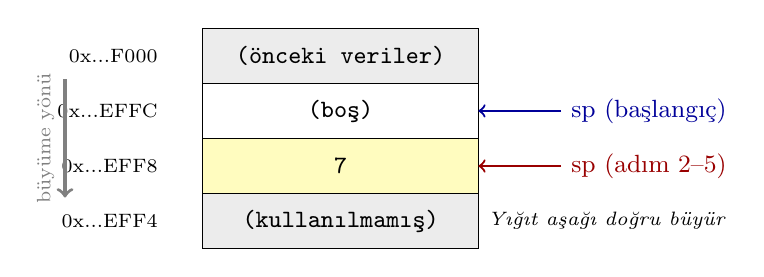
\begin{tikzpicture}[
    cell/.style={draw, minimum width=3.5cm, minimum height=0.7cm, font=\small\ttfamily},
    label/.style={font=\small, anchor=east},
    arrow/.style={->, thick, blue!60!black}
]
% High address (top)
\node[cell, fill=gray!15] (top) at (0,2.8) {(önceki veriler)};
\node[cell] (effc) at (0,2.1) {(boş)};
\node[cell, fill=yellow!25] (eff8) at (0,1.4) {7};
\node[cell, fill=gray!15] (low) at (0,0.7) {(kullanılmamış)};

% Addresses
\node[label] at (-2.2,2.8) {\scriptsize 0x...F000};
\node[label] at (-2.2,2.1) {\scriptsize 0x...EFFC};
\node[label] at (-2.2,1.4) {\scriptsize 0x...EFF8};
\node[label] at (-2.2,0.7) {\scriptsize 0x...EFF4};

% SP arrows
\draw[arrow] (2.8,2.1) -- (1.75,2.1) node[pos=0, right, font=\small] {sp (başlangıç)};
\draw[arrow, red!60!black] (2.8,1.4) -- (1.75,1.4) node[pos=0, right, font=\small, red!60!black] {sp (adım 2--5)};

% Growth direction
\draw[->, very thick, gray] (-3.5,2.5) -- (-3.5,1.0) node[midway, left, font=\scriptsize, rotate=90, anchor=south] {büyüme yönü};

% Label
\node[font=\scriptsize, anchor=west] at (1.75,0.7) {\emph{Yığıt aşağı doğru büyür}};
\end{tikzpicture}
\caption[Yığıt işaretçisinin yazmaç saklama sırasındaki değişimi]{Yığıt işaretçisinin yazmaç saklama sırasındaki değişimi. Sarı hücre \texttt{s0}'ın yığıtta saklanan değerini, oklar ise \texttt{sp}'nin hareket yönünü gösterir.}
\label{fig:yigit-buyume}
\end{figure}

Bu tablodaki kritik an 4.~ve 5.~adımlar arasıdır: \texttt{s0} geçici olarak 999 yapılmış olsa da yığıttaki eski değer (7) korunmaktadır. 5.~adımda \texttt{lw} bu değeri geri yükler. Yığıt işaretçisinin 2.~adımda düşüp 6.~adımda eski yerine döndüğüne de dikkat edin; her \texttt{addi sp, sp, -N} için karşılık gelen bir \texttt{addi sp, sp, +N} bulunmalıdır; aksi takdirde yığıt taşması oluşur.

\emph{Başarım çözümlemesi:} Yazdırma buyrukları dahil program 11 buyruk yürütür; 2'si bellek erişimi (\texttt{sw}, \texttt{lw}), 9'u yazmaç işlemidir. Yazmaç buyrukları 1, bellek buyrukları 2 çevrimle: $9 \times 1 + 2 \times 2 = 13$ çevrim, BBÇ~$= 13/11 \approx 1{,}18$. Bir yazmacı saklamak ve geri yüklemek için 4 fazladan buyruk (2 \texttt{addi} + 1 \texttt{sw} + 1 \texttt{lw}) gerektiğine dikkat edin; fonksiyon çağrılarında birden çok yazmacın saklanması bu ek yükü katlayacaktır.
\end{ornek}

\begin{karsilastirma}[Yığıt İşlemleri: RISC-V, x86 ve ARM]
RISC-V'te ayrı bir \texttt{push}/\texttt{pop} buyruğu yoktur; yığıt işaretçisini ayarlayıp \texttt{sw}/\texttt{lw} ile saklamak programcının sorumluluğundadır. Diğer mimariler bu konuda farklı tercihler yapmıştır:

\begin{center}
\small
\begin{tabular}{lll}
\toprule
İşlem & x86 & RISC-V \\
\midrule
Yığıta it & \texttt{push eax} \emph{(1 buyruk)} & \texttt{addi sp, sp, -4} \emph{(2 buyruk)} \\
 & & \texttt{sw s0, 0(sp)} \\
Yığıttan çek & \texttt{pop eax} \emph{(1 buyruk)} & \texttt{lw s0, 0(sp)} \emph{(2 buyruk)} \\
 & & \texttt{addi sp, sp, 4} \\
\bottomrule
\end{tabular}
\end{center}

ARM mimarisinde de \texttt{push} ve \texttt{pop} buyrukları bulunur; üstelik tek buyrukla birden çok yazmacı aynı anda saklayabilir: \texttt{push \{r4, r5, lr\}}.

Peki RISC-V neden özel yığıt buyrukları sunmaz? Çünkü \texttt{push}/\texttt{pop}, yalnızca \texttt{addi}~+~\texttt{sw}/\texttt{lw} birleşiminin kısaltmasıdır; ayrı bir buyruk olarak eklenmesi işlem kodu alanını tüketir ve çözücü donanımını karmaşıklaştırır. RISC-V ``basit olanı doğru yap'' felsefesine sadık kalarak bu görevi yazılıma bırakır. Bununla birlikte, RISC-V'in yeni \emph{Zcmp} uzantısı \texttt{cm.push} ve \texttt{cm.pop} sözde buyrukları ekleyerek bu boşluğu gömülü sistemler için doldurmaktadır.
\end{karsilastirma}

\begin{ornek}[4.4]
\label{orn:yigit-toplama}
Kullanıcıdan iki sayı alın, her birini yığıta itin (\emph{push}), ardından yığıttan çıkararak (\emph{pop}) toplayın ve sonucu yazdırın.

\textbf{Çözüm:}

\begin{lstlisting}[style=riscv]
.data
mesaj1:  .string "Birinci sayı: "
mesaj2:  .string "İkinci sayı: "

.text
.globl main
main:
    # Birinci sayıyı oku
    la   a0, mesaj1
    li   a7, 4                # 4 = karakter dizisi yazdır
    ecall
    li   a7, 5                # 5 = tam sayı oku
    ecall
    mv   t0, a0               # t0 = birinci sayı

    # Birinci sayıyı yığıta it
    addi sp, sp, -4
    sw   t0, 0(sp)

    # İkinci sayıyı oku
    la   a0, mesaj2
    li   a7, 4
    ecall
    li   a7, 5
    ecall
    mv   t1, a0               # t1 = ikinci sayı

    # İkinci sayıyı yığıta it
    addi sp, sp, -4
    sw   t1, 0(sp)

    # Yığıttan iki değeri çıkar ve topla
    lw   t1, 0(sp)            # t1 = ikinci sayı (son giren)
    addi sp, sp, 4
    lw   t0, 0(sp)            # t0 = birinci sayı
    addi sp, sp, 4

    add  a0, t0, t1           # a0 = toplam
    li   a7, 1
    ecall

    li   a7, 10
    ecall
\end{lstlisting}

Yığıt LIFO (\emph{Last In, First Out}, yani son giren ilk çıkar) düzeninde çalışır. İlk itilen değer altta, son itilen değer üstte kalır. RARS'ta bu programı adım adım yürütürken, yığıt alanında iki değerin nasıl biriktiğini ve sonra nasıl geri alındığını gözlemleyin. Bu örüntü (değer sakla, başka işler yap, geri yükle) çevirici dil programlamanın temel yapı taşıdır ve fonksiyon çağrılarında yaygın biçimde kullanılır.

\emph{Başarım çözümlemesi:} Buyrukları sayalım: \texttt{la} $\times 2$, \texttt{li} $\times 6$, \texttt{mv} $\times 2$, \texttt{addi} $\times 4$, \texttt{sw} $\times 2$, \texttt{lw} $\times 2$, \texttt{add} $\times 1$, \texttt{ecall} $\times 6$: toplam 25 buyruk. 4'ü bellek erişimi (\texttt{sw} $\times 2$, \texttt{lw} $\times 2$), 21'i yazmaç veya sistem çağrısıdır. Yazmaç buyrukları 1, bellek buyrukları 2 çevrimle: $21 \times 1 + 4 \times 2 = 29$ çevrim, BBÇ~$= 29/25 = 1{,}16$. Dört örnekteki BBÇ değerlerini yan yana koyalım: 1{,}00 $\rightarrow$ 1{,}20 $\rightarrow$ 1{,}18 $\rightarrow$ 1{,}16. Bellek erişim oranı düştükçe BBÇ 1{,}0'a yaklaşır; bu programda buyruk sayısı artmasına karşın bellek erişim oranı (\%16) düşük kaldığından BBÇ nispeten iyidir. Bölüm~\ref{chap:basarim}'deki yürütme süresi formülünü hatırlayın: $T = N \times \text{BBÇ} \times T_{\text{çevrim}}$; BBÇ'yi düşürmek başarımı doğrudan artırır.
\end{ornek}

\subsection{Döngüler}
\label{subsec:donguler}

Önceki örneklerde tüm buyruklar yalnızca bir kez yürütülüyordu; bu nedenle durağan ve devingen buyruk sayıları birbirine eşitti. Döngü kullandığımızda bu durum değişir: aynı buyruklar defalarca yürütülür ve devingen buyruk sayısı durağan sayıdan çok daha büyük olabilir.

\begin{ornek}[4.5]
\label{orn:dongu-toplam}
1'den 10'a kadar tam sayıların toplamını ($1 + 2 + \ldots + 10 = 55$) bir döngüyle hesaplayın.

\textbf{Çözüm:}

\begin{lstlisting}[style=riscv]
.text
.globl main
main:
    li   t0, 0                # toplam = 0
    li   t1, 1                # i = 1
    li   t2, 10               # üst sınır
dongu:
    add  t0, t0, t1           # toplam += i
    addi t1, t1, 1            # i++
    ble  t1, t2, dongu        # i <= 10 ise tekrarla

    mv   a0, t0               # sonucu yazdır
    li   a7, 1
    ecall
    li   a7, 10
    ecall
\end{lstlisting}

Bu programda \texttt{ble} (\emph{branch if less than or equal}, küçükse veya eşitse dallan) buyruğu, \texttt{t1~$\leq$~t2} koşulunu sağladığı sürece \texttt{dongu} etiketine geri döndürür. Yazmaç izleme tablosunun ilk birkaç yinelemesine bakalım:

\begin{center}
\small
\begin{tabular}{clcccl}
\toprule
\texttt{\#} & Buyruk & \texttt{t0} & \texttt{t1} & \texttt{t2} & Dallanma \\
\midrule
  & \emph{(başlangıç)} & 0 & 0 & 0 & --- \\
1 & \texttt{addi t0, x0, 0} & \underline{0} & 0 & 0 & --- \\
2 & \texttt{addi t1, x0, 1} & 0 & \underline{1} & 0 & --- \\
3 & \texttt{addi t2, x0, 10} & 0 & 1 & \underline{10} & --- \\
\midrule
\multicolumn{6}{c}{\emph{1.~yineleme}} \\
4 & \texttt{add t0, t0, t1} & \underline{1} & 1 & 10 & --- \\
5 & \texttt{addi t1, t1, 1} & 1 & \underline{2} & 10 & --- \\
6 & \texttt{ble t1, t2, dongu} & 1 & 2 & 10 & $2 \leq 10$: dallan \\
\midrule
\multicolumn{6}{c}{\emph{2.~yineleme}} \\
7 & \texttt{add t0, t0, t1} & \underline{3} & 2 & 10 & --- \\
8 & \texttt{addi t1, t1, 1} & 3 & \underline{3} & 10 & --- \\
9 & \texttt{ble t1, t2, dongu} & 3 & 3 & 10 & $3 \leq 10$: dallan \\
\midrule
\multicolumn{6}{c}{$\vdots$ \quad (10.~yinelemede \texttt{t0}~=~55, \texttt{t1}~=~11)} \\
\midrule
\multicolumn{6}{c}{\emph{10.~yineleme (son)}} \\
31 & \texttt{add t0, t0, t1} & \underline{55} & 10 & 10 & --- \\
32 & \texttt{addi t1, t1, 1} & 55 & \underline{11} & 10 & --- \\
33 & \texttt{ble t1, t2, dongu} & 55 & 11 & 10 & $11 \leq 10$: \emph{hayır} \\
\bottomrule
\end{tabular}
\end{center}

Bu örnekte durağan ve devingen buyruk sayıları arasındaki fark ilk kez belirgin biçimde ortaya çıkar:

\begin{center}
\small
\begin{tabular}{lcc}
\toprule
Buyruk türü & Sayı & Hesaplama \\
\midrule
Durağan (bellekteki buyruklar) & 10 & Döngü gövdesi yalnızca bir kez saklanır \\
Devingen (yürütülen toplam) & 37 & $3 + 3 \times 10 + 4 = 37$ \\
\bottomrule
\end{tabular}
\end{center}

Devingen sayının hesabı: 3 başlangıç buyruğu (\texttt{li} $\times 3$) + döngü gövdesindeki 3 buyruk $\times$ 10 yineleme + 4 son buyruk (\texttt{mv}, \texttt{li}, \texttt{ecall} $\times 2$). Döngü gövdesindeki 3 buyruktan hiçbiri bellek erişimi değildir (\texttt{ble} bir dallanma buyruğudur, bellek erişimi değil).

\emph{Başarım çözümlemesi:} 37 devingen buyruktan hiçbiri bellek erişimi değildir (\texttt{lw}/\texttt{sw} yok); tümü yazmaç işlemi veya dallanmadır. Her buyruk tek çevrimde tamamlansa BBÇ~$= 1{,}0$ olur. Dallanma buyrukları bazı durumlarda ek çevrimlere neden olabilir; bu konuyu Bölüm~\ref{chap:boruhatti}'de ayrıntılı olarak ele alacağız. Şimdilik her buyruğun tek çevrimde tamamlandığını varsayarsak $37 \times 1 = 37$ çevrim ve BBÇ~$= 1{,}0$ elde ederiz. Önceki örneklerle karşılaştırın: bellek erişimi olan programlarda BBÇ~$\sim$1{,}2'ye çıkıyordu; bu programda bellek erişimi olmadığından BBÇ en iyi değerinde kalmaktadır.
\end{ornek}

\begin{ornek}[4.6]
\label{orn:altyordam-cagirma}
Verilen iki sayının toplamını hesaplayan bir \emph{altyordam} (\emph{subroutine}) yazın. Ana program bu altyordamı çağırsın ve sonucu ekrana yazdırsın.

\textbf{Çözüm:}

\begin{lstlisting}[style=riscv]
.text
.globl main
main:
    li   a0, 30               # birinci argüman
    li   a1, 12               # ikinci argüman
    jal  topla                 # altyordamı çağır

    # a0 artık dönüş değerini tutar (42)
    li   a7, 1
    ecall
    li   a7, 10
    ecall

# topla: a0 + a1 hesapla, sonucu a0'da döndür
topla:
    add  a0, a0, a1           # a0 = a0 + a1
    ret                        # çağırana geri dön
\end{lstlisting}

\texttt{jal} (\emph{jump and link}, atla ve bağla) buyruğu iki iş yapar: (1)~bir sonraki buyruğun adresini \texttt{ra} (\emph{return address}, dönüş adresi) yazmacına kaydeder; (2)~\texttt{topla} etiketine atlar. \texttt{ret} ise \texttt{ra}'daki adrese geri döner. Bu mekanizma sayesinde bir altyordam birden çok yerden çağrılabilir ve her seferinde doğru yere geri döner.

\texttt{topla} altyordamı \emph{yaprak fonksiyondur} (\emph{leaf function}): başka fonksiyon çağırmaz. Bu nedenle \texttt{ra}'yı yığıtta saklamasına gerek yoktur, çünkü kendi \texttt{ra} değerini bozacak bir \texttt{jal} çağrısı yapmaz. Yaprak olmayan fonksiyonlarda (bir fonksiyonun başka bir fonksiyonu çağırdığı durumda) \texttt{ra} yığıtta saklanmalıdır; bu durumu Örnek~4.8'de göreceğiz.

Yazmaç izleme tablosu:

\begin{center}
\small
\begin{tabular}{clcccc}
\toprule
\texttt{\#} & Buyruk & \texttt{a0} & \texttt{a1} & \texttt{ra} & PC \\
\midrule
  & \emph{(başlangıç)} & 0 & 0 & 0 & \texttt{main} \\
1 & \texttt{addi a0, x0, 30} & \underline{30} & 0 & 0 & \texttt{main+4} \\
2 & \texttt{addi a1, x0, 12} & 30 & \underline{12} & 0 & \texttt{main+8} \\
3 & \texttt{jal topla} & 30 & 12 & \underline{\texttt{main+12}} & \underline{\texttt{topla}} \\
\midrule
\multicolumn{6}{c}{\emph{(altyordamın içinde)}} \\
4 & \texttt{add a0, a0, a1} & \underline{42} & 12 & \texttt{main+12} & \texttt{topla+4} \\
5 & \texttt{jalr x0, ra, 0} (ret) & 42 & 12 & \texttt{main+12} & \underline{\texttt{main+12}} \\
\midrule
\multicolumn{6}{c}{\emph{(ana programa dönüş)}} \\
6 & \texttt{addi a7, x0, 1} & 42 & 12 & \texttt{main+12} & \texttt{main+16} \\
7 & \texttt{ecall} & 42 & 12 & \texttt{main+12} & \texttt{main+20} \\
\bottomrule
\end{tabular}
\end{center}

\begin{figure}[H]
\centering
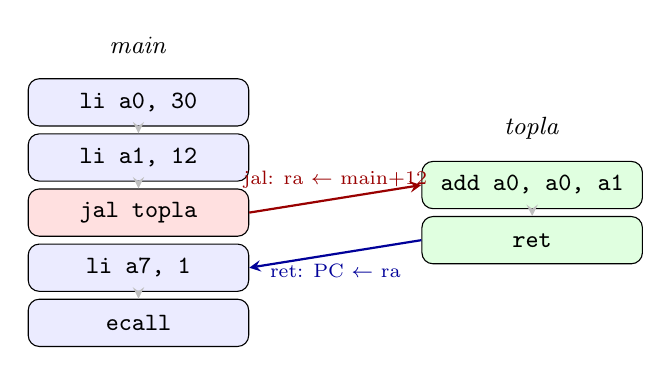
\begin{tikzpicture}[
    box/.style={draw, rounded corners, minimum width=2.8cm, minimum height=0.6cm, font=\small\ttfamily, fill=#1},
    box/.default=blue!8,
    arrow/.style={->, thick, >=stealth}
]
% Main program
\node[box=blue!8] (li1) at (0,3.5) {li a0, 30};
\node[box=blue!8] (li2) at (0,2.8) {li a1, 12};
\node[box=red!12] (jal) at (0,2.1) {jal topla};
\node[box=blue!8] (li3) at (0,1.4) {li a7, 1};
\node[box=blue!8] (ecall) at (0,0.7) {ecall};

% Subroutine
\node[box=green!12] (add) at (5,2.45) {add a0, a0, a1};
\node[box=green!12] (ret) at (5,1.75) {ret};

% Labels
\node[font=\small, anchor=south] at (0,4.0) {\emph{main}};
\node[font=\small, anchor=south] at (5,2.9) {\emph{topla}};

% Arrows
\draw[arrow, red!60!black] (jal.east) -- (add.west) node[midway, above, font=\scriptsize] {jal: ra $\leftarrow$ main+12};
\draw[arrow, blue!60!black] (ret.west) -- (li3.east) node[midway, below, font=\scriptsize] {ret: PC $\leftarrow$ ra};

% Sequential arrows
\draw[arrow, gray!50] (li1) -- (li2);
\draw[arrow, gray!50] (li2) -- (jal);
\draw[arrow, gray!50] (li3) -- (ecall);
\draw[arrow, gray!50] (add) -- (ret);
\end{tikzpicture}
\caption[Altyordam çağrısında kontrol akışı]{Altyordam çağrısında kontrol akışı. \texttt{jal} buyruğu PC'yi altyordama yönlendirirken \texttt{ra}'ya dönüş adresini yazar; \texttt{ret} ise \texttt{ra}'daki adrese geri döner.}
\label{fig:altyordam-akis}
\end{figure}

Tablodaki kritik satırlar 3.~ve 5.~adımlardır: \texttt{jal} PC'yi \texttt{topla}'ya yönlendirirken \texttt{ra}'ya dönüş adresini yazar; \texttt{ret} ise PC'yi \texttt{ra}'daki adrese geri getirir. PC sütunundaki gidiş-dönüş hareketini izlemek, altyordam mekanizmasını kavramanın en somut yoludur.

\emph{Başarım çözümlemesi:} Program 9 buyruk yürütür (sözde buyruklar açıldığında). Tümü yazmaç işlemidir; bellek erişimi yoktur. \texttt{jal} ve \texttt{ret} buyrukları da birer çevrimde tamamlanır; altyordam çağırmanın kendisi ek maliyet getirmez. Asıl maliyet, yaprak olmayan fonksiyonlarda \texttt{ra}'yı ve saklanan yazmaçları yığıtta koruma zorunluluğundan doğar: Örnek~4.3'te gördüğümüz gibi her \texttt{sw}/\texttt{lw} çifti BBÇ'yi artırır.
\end{ornek}

\begin{bilginot}[RARS'ta Adım Adım Yürütme]
Yukarıdaki örnekleri anlamanın en etkili yolu, RARS benzeticisinde adım adım (\emph{single step}) çalıştırmaktır. Her buyruktan sonra üç şeyi kontrol edin: (1)~hangi yazmaçların değeri değişti, (2)~bellek içeriği nasıl etkilendi ve (3)~program sayacı (PC) hangi buyruğa ilerledi. Dallanma buyrukları çalıştığında PC'nin sıradaki buyruğa değil, etiketin gösterdiği adrese atladığını gözlemlemek, kontrol akışını kavramanın en somut yoludur.
\end{bilginot}

\begin{bilginot}[Programlama ve Başarım İlişkisi]
Bu bölümdeki her örnekte başarım çözümlemesi yaptık. Buyruk başına çevrim (BBÇ) değerini etkileyen iki temel etken gördük: (1)~bellek erişimi: \texttt{lw}/\texttt{sw} buyrukları yazmaç işlemlerinden daha fazla çevrim alır; (2)~dallanma buyrukları: bazı durumlarda ek çevrimlere neden olabilir (nedenini Bölüm~\ref{chap:boruhatti}'de göreceğiz). Bölüm~\ref{chap:basarim}'deki formülü hatırlayın:
\[
T_{\text{yürütme}} = N_{\text{buyruk}} \times \text{BBÇ} \times T_{\text{çevrim}}
\]
Bir programı hızlandırmanın üç yolu bu formülde gizlidir: buyruk sayısını azaltmak (daha iyi algoritma), BBÇ'yi düşürmek (bellek erişimini en aza indirmek) veya çevrim süresini kısaltmak (daha yüksek saat sıklığı). Programcı olarak ilk iki etken üzerinde doğrudan kontrolümüz vardır.
\end{bilginot}

\begin{terimnotu}
\textbf{gömülü sistem} (\emph{embedded system})\,: \emph{Gömmek} fiilinden \emph{-ülü} ekiyle; genel amaçlı olmayan, belirli bir görevi yerine getirmek üzere donanımın içine ``gömülmüş'' bilgisayar sistemidir.

\textbf{döngü açma} (\emph{loop unrolling})\,: Döngü gövdesini birden çok kez tekrarlayarak dallanma buyrukları sayısını azaltan bir eniyileme tekniğidir. ``Açma'' sözcüğü, katlanmış (döngülenmiş) kodun düz bir çizgiye açılmasını ifade eder.

\textbf{özyineleme} (\emph{recursion})\,: \emph{Öz} (self) ve \emph{yineleme} (iteration) sözcüklerinin birleşimi; bir fonksiyonun kendisini çağırması anlamına gelir. Latince \emph{recurrere} (geri koşmak) kökünden gelen İngilizce terimin Türkçe karşılığıdır.
\end{terimnotu}


% =====================================================
\section{Program Yapısı ve Geliştirme Ortamı}
\label{sec:program-yapisi}
\index{RISC-V!programlama}

\subsection{Bir RISC-V Programının Anatomisi}
\label{subsec:program-anatomisi}

Bir RISC-V çevirici dil programı, temelde üç bölümden oluşur: \emph{veri bölümü} (\texttt{.data}), \emph{metin bölümü} (\texttt{.text}) ve isteğe bağlı olarak \emph{salt okunur veri bölümü} (\texttt{.rodata}). Metin bölümü programın buyruklarını, veri bölümü ise program tarafından kullanılan değişkenleri ve sabitleri barındırır.

\begin{lstlisting}[style=riscv]
.data                        # Veri bölümü
ileti: .asciz "Merhaba!\n"   # Karakter dizisi
sayi:  .word  42             # 32 bitlik tam sayı
dizi:  .word  5, 3, 8, 1, 9  # 5 elemanlı dizi

.text                        # Metin (kod) bölümü
.globl main                  # Giriş noktasını dışa aç
main:
    # Program burada başlar
    la   a0, ileti            # ileti adresini yükle
    li   a7, 4                # yazdırma sistem çağrısı
    ecall                     # işletim sistemini çağır

    li   a7, 10               # çıkış sistem çağrısı
    ecall                     # programı sonlandır
\end{lstlisting}

\index{veri bölümü}\index{metin bölümü}
Bu programı adım adım inceleyelim. Program iki ana bölümden oluşur: \texttt{.data} ve \texttt{.text}. Veri bölümünde (\texttt{.data}) üç değişken tanımlanmıştır: \texttt{ileti} adlı bir karakter dizisi, \texttt{sayi} adlı 32 bitlik bir tam sayı ve \texttt{dizi} adlı beş elemanlı bir dizi. Bu değişkenler belleğin veri kesiminde (\emph{data segment}) yer alır.

Metin bölümünde (\texttt{.text}) programın buyrukları bulunur. \texttt{.globl main} yönergesi, \texttt{main} etiketinin bağlayıcı (\emph{linker}) tarafından görülebilmesini sağlar; bu, programın giriş noktasıdır. İlk buyruk \texttt{la a0, ileti} ile karakter dizisinin bellek adresi \texttt{a0} yazmacına yüklenir. Ardından \texttt{li a7, 4} ile sistem çağrısı numarası belirlenir ve \texttt{ecall} buyruğuyla işletim sistemi çağrılarak karakter dizisi ekrana yazdırılır. Son iki satırda \texttt{a7} yazmacına 10 değeri yüklenerek programdan çıkış yapılır.

Veri bölümünde kullanılan yönergeler şunlardır:

\begin{table}[H]
\centering
\caption{Veri tanımlama yönergeleri}
\label{tab:veri-yonergeleri}
\small
\begin{tabularx}{\textwidth}{l l X}
\toprule
\textbf{Yönerge} & \textbf{Boyut} & \textbf{Açıklama} \\
\midrule
\texttt{.byte} & 1 bayt & 8 bitlik tam sayı \\
\texttt{.half} & 2 bayt & 16 bitlik tam sayı \\
\texttt{.word} & 4 bayt & 32 bitlik tam sayı \\
\texttt{.dword} & 8 bayt & 64 bitlik tam sayı (RV64) \\
\texttt{.asciz} & değişken & Sıfır ile sonlandırılmış karakter dizisi \\
\texttt{.string} & değişken & \texttt{.asciz} ile aynı \\
\texttt{.space} $n$ & $n$ bayt & $n$ baytlık sıfırlanmış alan ayırma \\
\texttt{.align} $n$ & -- & Sonraki veriyi $2^n$ bayt sınırına hizalama \\
\bottomrule
\end{tabularx}
\end{table}

\begin{figure}[H]
\centering
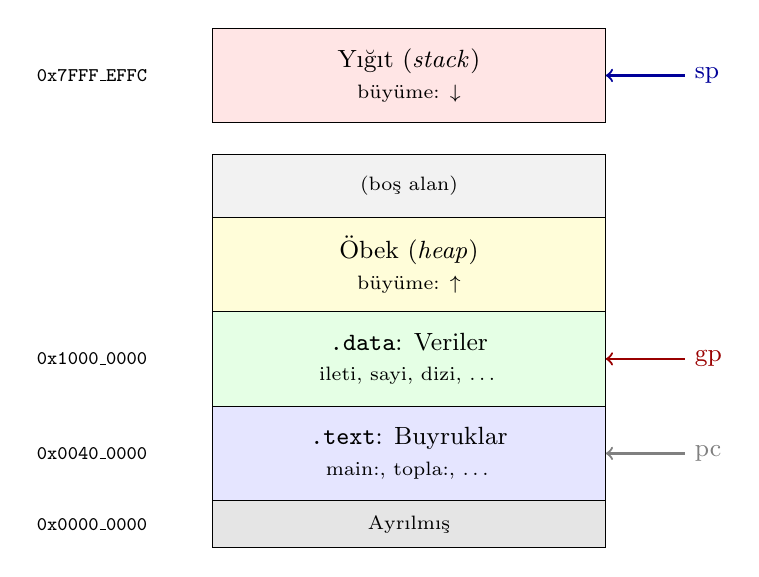
\begin{tikzpicture}[
    segment/.style={draw, minimum width=5cm, minimum height=1.2cm, font=\small, align=center},
    addr/.style={font=\scriptsize\ttfamily, anchor=east}
]
% Memory segments (top = high address)
\node[segment, fill=red!10] (stack) at (0,5.4) {Yığıt (\emph{stack})\\{\scriptsize büyüme: $\downarrow$}};
\node[segment, fill=gray!10, minimum height=0.8cm] (free) at (0,4.0) {\scriptsize (boş alan)};
\node[segment, fill=yellow!15] (heap) at (0,3.0) {Öbek (\emph{heap})\\{\scriptsize büyüme: $\uparrow$}};
\node[segment, fill=green!10] (data) at (0,1.8) {\texttt{.data}: Veriler\\{\scriptsize ileti, sayi, dizi, \ldots}};
\node[segment, fill=blue!10] (text) at (0,0.6) {\texttt{.text}: Buyruklar\\{\scriptsize main:, topla:, \ldots}};
\node[segment, fill=gray!20, minimum height=0.6cm] (res) at (0,-0.3) {\scriptsize Ayrılmış};

% Addresses
\node[addr] at (-3.2,5.4) {0x7FFF\_EFFC};
\node[addr] at (-3.2,1.8) {0x1000\_0000};
\node[addr] at (-3.2,0.6) {0x0040\_0000};
\node[addr] at (-3.2,-0.3) {0x0000\_0000};

% SP and GP labels
\draw[->, thick, blue!60!black] (3.5,5.4) -- (2.5,5.4) node[pos=0, right, font=\small] {sp};
\draw[->, thick, red!60!black] (3.5,1.8) -- (2.5,1.8) node[pos=0, right, font=\small] {gp};
\draw[->, thick, gray] (3.5,0.6) -- (2.5,0.6) node[pos=0, right, font=\small] {pc};
\end{tikzpicture}
\caption[RISC-V programının bellek düzeni]{RISC-V programının bellek düzeni. Yığıt yüksek adreslerden aşağıya doğru büyürken öbek düşük adreslerden yukarıya doğru büyür.}
\label{fig:bellek-duzeni}
\end{figure}

\subsection{Geliştirme Ortamı}
\label{subsec:gelistirme-ortami}
\index{RARS}\index{Venus}

RISC-V çevirici dil programlarını denemek ve çalıştırmak için çeşitli araçlar kullanılabilir. Bu kitapta örnekler için RARS (\emph{RISC-V Assembler and Runtime Simulator}) benzetimliği kullanılmıştır. RARS, Java tabanlı bir grafik arayüze sahiptir ve programları adım adım çalıştırma, yazmaç ve bellek içeriklerini izleme gibi olanaklar sunar. Tarayıcı tabanlı bir seçenek olarak Venus de kullanılabilir. Her iki aracın ayrıntılı kurulum ve kullanım bilgileri Ek~D'de verilmiştir.

\begin{bilginot}[Sistem Çağrıları]
RARS benzetimliğinde \texttt{ecall} buyruğu, \texttt{a7} yazmacındaki değere göre farklı sistem çağrıları gerçekleştirir: 1 = tam sayı yazdır, 4 = karakter dizisi yazdır, 5 = tam sayı oku, 10 = programı sonlandır, 11 = karakter yazdır. Gerçek bir RISC-V sisteminde bu çağrılar işletim sistemi çekirdeği tarafından işlenir ve numaralandırma farklıdır.
\end{bilginot}


% =====================================================
\section{Algoritmalar ve Veri Yapıları}
\label{sec:algoritmalar}
\index{RISC-V!algoritmalar}

Temel yazmaç ve bellek işlemlerini öğrendikten sonra, şimdi bu becerileri gerçek problemlere uygulayalım. Bu bölümde dizilerde arama ve sıralama, karakter dizisi işleme ve yapılarla çalışma konularını ele alacağız.

\subsection{Dizilerde Doğrusal Arama}
\label{subsec:dogrusal-arama}
\index{doğrusal arama}\index{linear search|see{doğrusal arama}}

Doğrusal arama, bir dizideki elemanları baştan sona tek tek kontrol ederek aranan değeri bulmaya çalışır. Basit ama öğretici bir örnektir: döngü, bellek erişimi, karşılaştırma ve dallanma buyruklarının hepsini bir arada kullanır.

\begin{ornek}[4.7]
\label{orn:dogrusal-arama}
Bellekteki bir tam sayı dizisinde verilen bir değeri arayan ve bulursa dizin numarasını, bulamazsa $-1$ döndüren bir RISC-V programı yazın.

\textbf{Çözüm:} Önce bu algoritmayı C dilinde ifade edelim, ardından RISC-V çevirici diline dönüştürelim:

\begin{lstlisting}[language=C, style=alistirma-kod]
int dogrusal_ara(int dizi[], int boyut, int aranan) {
    for (int i = 0; i < boyut; i++) {
        if (dizi[i] == aranan)
            return i;
    }
    return -1;
}
\end{lstlisting}

Şimdi bu fonksiyonu RISC-V çevirici dilinde yazalım. Çağrı düzenine uygun olarak \texttt{a0} = dizi adresi, \texttt{a1} = boyut, \texttt{a2} = aranan değer, dönüş değeri \texttt{a0}'da olacaktır:

\begin{lstlisting}[style=riscv]
# a0=dizi adresi, a1=boyut, a2=aranan
# Dönüş: a0 = bulunan dizin veya -1
dogrusal_ara:
    li   t0, 0                # t0 = i = 0
dongu:
    bge  t0, a1, bulunamadi   # i >= boyut ise çık
    slli t1, t0, 2            # t1 = i * 4 (bayt uzaklığı)
    add  t1, a0, t1           # t1 = dizi + i*4
    lw   t2, 0(t1)            # t2 = dizi[i]
    beq  t2, a2, bulundu      # dizi[i] == aranan ise atla
    addi t0, t0, 1            # i++
    j    dongu                # döngüye devam
bulundu:
    mv   a0, t0               # dönüş değeri = i
    ret
bulunamadi:
    li   a0, -1               # dönüş değeri = -1
    ret
\end{lstlisting}

Bu programda \texttt{slli t0, t0, 2} buyruğu dizin numarasını bayt uzaklığına çevirir. Her \texttt{.word} 4 bayt olduğu için dizin $i$, bellekte $i \times 4$ bayt ileridedir.

\emph{Başarım çözümlemesi:} Döngü gövdesi 7 buyruktan oluşur (\texttt{bge}, \texttt{slli}, \texttt{add}, \texttt{lw}, \texttt{beq}, \texttt{addi}, \texttt{j}); bunların 1'i bellek erişimi (\texttt{lw}), 2'si dallanma buyruğudur. $n$ elemanlı bir dizide aranan değer bulunamazsa döngü $n$ kez yinelenir: toplam $7n + 2$ buyruk (giriş ve çıkış dahil). Yazmaç buyrukları 1, bellek buyrukları 2, dallanma buyrukları 2 çevrimle bir yineleme $3 \times 1 + 1 \times 2 + 2 \times 2 + 1 \times 1 = 8$ çevrim alır. $n = 100$ için: toplam $\sim$702 buyruk, $\sim$802 çevrim, BBÇ~$\approx 1{,}14$. Bellek erişiminin döngü başına yalnızca 1 kez yapılması BBÇ'yi düşük tutar, ancak arama başarısız olursa $n$'e orantılı buyruk yürütülür. Bölüm~\ref{chap:basarim}'deki asimptotik karmaşıklık kavramını hatırlayın: bu algoritma $O(n)$ zamanda çalışır.
\end{ornek}


Doğrusal arama, bir dizide tek geçişle eleman bulmayı gösterdi. Peki ya diziyi önce sıralamamız gerekirse? Sıralı bir dizide ikili arama $O(\log n)$ zamanda çalışır; ancak sıralama işleminin kendisi en az $O(n \log n)$ zaman alır. Şimdi en basit sıralama algoritmalarından birini çevirici dilde yazarak iç içe döngülerin ve yer değiştirme (\emph{swap}) işleminin nasıl gerçekleştirildiğini görelim.

\subsection{Kabarcık Sıralama}
\label{subsec:kabarcik-siralama}
\index{kabarcık sıralama}\index{bubble sort|see{kabarcık sıralama}}

Kabarcık sıralama, ardışık elemanları karşılaştırarak gerektiğinde yer değiştiren yalın bir sıralama algoritmasıdır. Başarımı $O(n^2)$ olsa da çevirici dilde yazması kolaydır ve bellek erişim kalıplarını anlamak için iyi bir örnektir.

\begin{ornek}[4.8]
\label{orn:kabarcik-siralama}
Bellekteki bir tam sayı dizisini küçükten büyüğe sıralayan bir RISC-V kabarcık sıralama programı yazın.

\textbf{Çözüm:} C dilindeki karşılığı:

\begin{lstlisting}[language=C, style=alistirma-kod]
void kabarcik_sirala(int dizi[], int boyut) {
    for (int i = 0; i < boyut - 1; i++)
        for (int j = 0; j < boyut - 1 - i; j++)
            if (dizi[j] > dizi[j+1]) {
                int gecici = dizi[j];
                dizi[j] = dizi[j+1];
                dizi[j+1] = gecici;
            }
}
\end{lstlisting}

RISC-V çevirici dili karşılığı (\texttt{a0} = dizi adresi, \texttt{a1} = boyut):

\begin{lstlisting}[style=riscv]
# kabarcik\_sirala: a0=dizi adresi, a1=boyut
kabarcik_sirala:
    addi sp, sp, -20          # yığıtta yer aç
    sw   ra, 16(sp)           # dönüş adresini sakla
    sw   s0, 12(sp)           # s0'ı sakla
    sw   s1, 8(sp)            # s1'i sakla
    sw   s2, 4(sp)            # s2'yi sakla
    sw   s3, 0(sp)            # s3'ü sakla
    mv   s0, a0               # s0 = dizi adresi
    mv   s1, a1               # s1 = boyut

    li   t0, 0                # t0 = i = 0
    addi t3, s1, -1           # t3 = boyut - 1
dis_dongu:
    bge  t0, t3, son          # i >= boyut-1 ise bitir
    sub  t4, t3, t0           # t4 = boyut - 1 - i
    li   t1, 0                # t1 = j = 0
ic_dongu:
    bge  t1, t4, dis_devam    # j >= boyut-1-i ise dış döngüye
    slli t5, t1, 2            # t5 = j * 4
    add  t5, s0, t5           # t5 = \&dizi[j]
    lw   s2, 0(t5)            # s2 = dizi[j]
    lw   s3, 4(t5)            # s3 = dizi[j+1]
    ble  s2, s3, degistirme   # dizi[j] <= dizi[j+1] ise atla
    sw   s3, 0(t5)            # dizi[j] = dizi[j+1]
    sw   s2, 4(t5)            # dizi[j+1] = dizi[j]
degistirme:
    addi t1, t1, 1            # j++
    j    ic_dongu
dis_devam:
    addi t0, t0, 1            # i++
    j    dis_dongu
son:
    lw   s3, 0(sp)            # s3'ü geri yükle
    lw   s2, 4(sp)            # s2'yi geri yükle
    lw   s1, 8(sp)            # s1'i geri yükle
    lw   s0, 12(sp)           # s0'ı geri yükle
    lw   ra, 16(sp)           # dönüş adresini geri yükle
    addi sp, sp, 20           # yığıtı geri al
    ret
\end{lstlisting}

Bu programda dikkat çekilmesi gereken noktalar:
\begin{itemize}
\item Fonksiyon giriş kodunda (\emph{prologue}) saklanan yazmaçlar (\texttt{s0}--\texttt{s3}) ve dönüş adresi (\texttt{ra}) yığıta kaydedilir; çıkış kodunda (\emph{epilogue}) geri yüklenir. Bu, Bölüm~\ref{chap:buyruk-kumesi}'te gördüğümüz çağrı düzeninin doğrudan uygulamasıdır.
\item Dizi erişiminde \texttt{slli} ile dizin bayt uzaklığına çevrilir, ardından \texttt{lw}/\texttt{sw} ile bellek okunur/yazılır.
\item İç döngüde iki ardışık eleman (\texttt{0(t5)} ve \texttt{4(t5)}) okunarak karşılaştırılır. Yer değiştirme için üçüncü bir değişken (fazladan yazmaç) kullanılır.
\end{itemize}

\emph{Başarım çözümlemesi:} İç döngü gövdesi 9 buyruktan oluşur; bunların 2'si okuma (\texttt{lw}), yer değiştirme durumunda 2'si yazma (\texttt{sw}) olmak üzere 4 bellek erişimi içerir. $n$ elemanlı bir dizi için iç döngü toplam $n(n-1)/2$ kez yinelenir. $n = 10$ için 45 yineleme, her biri $\sim$13 çevrim (en kötü durumda): toplam $\sim$585 çevrim $+$ dış döngü ek yükü. BBÇ $\approx 1{,}4$ civarındadır; bellek erişiminin yoğun olduğu bu algoritmada BBÇ doğrusal aramaya göre belirgin biçimde yükselir. Ayrıca $O(n^2)$ karmaşıklık, $n$ büyüdükçe buyruk sayısının karesel artması demektir: $n = 100$ için $\sim$45.000 buyruk, $n = 1000$ için $\sim$4{,}5 milyon. Sıralama algoritmalarında verimlilik seçimi başarımı temelden etkiler.
\end{ornek}


Dizi üzerinde arama ve sıralama yaparken \texttt{lw}/\texttt{sw} ile 4 baytlık sözcükler üzerinde çalıştık. Ancak metin işleme, bayt bayt erişim gerektirir: her ASCII karakter 1 bayttır ve diziler sıfır (\texttt{0x00}) ile sonlandırılır. Şimdi \texttt{lb}/\texttt{sb} buyrukları ile karakter dizisi işleme fonksiyonları yazacağız.

\subsection{Karakter Dizisi İşleme}
\label{subsec:karakter-dizisi}
\index{karakter dizisi}\index{dizgi|see{karakter dizisi}}\index{string|see{karakter dizisi}}

Karakter dizileri (\emph{string}), kısaca \emph{dizgi} de denir; bellekte ardışık baytlar olarak saklanır ve sıfır (\texttt{0x00}) ile sonlandırılır. Bu tür verilere erişim, \texttt{lb} (\emph{load byte}, bayt yükle) ve \texttt{sb} (\emph{store byte}, bayt sakla) buyruklarıyla yapılır.

\begin{ornek}[4.9]
\label{orn:strlen}
Bir karakter dizisinin uzunluğunu hesaplayan \texttt{strlen} fonksiyonunu RISC-V çevirici dilinde yazın.

\textbf{Çözüm:}

\begin{lstlisting}[style=riscv]
# strlen: a0 = karakter dizisi adresi
# Dönüş: a0 = uzunluk
strlen:
    mv   t0, a0               # t0 = geçici işaretçi
    li   t1, 0                 # t1 = sayaç = 0
strlen_dongu:
    lb   t2, 0(t0)            # t2 = geçerli karakter
    beqz t2, strlen_son       # sıfır ise bitir
    addi t0, t0, 1            # işaretçiyi ilerlet
    addi t1, t1, 1            # sayacı artır
    j    strlen_dongu
strlen_son:
    mv   a0, t1               # dönüş değeri = uzunluk
    ret
\end{lstlisting}

Burada \texttt{lb} buyruğu 1 baytlık veri yükler (işaretle genişleterek); \texttt{lbu} ise işaretsiz genişletme yapar. ASCII karakterler 0--127 aralığında olduğu için her ikisi de aynı sonucu verir.
\end{ornek}

\begin{ornek}[4.10]
\label{orn:strcpy}
Bir karakter dizisini başka bir bellek alanına kopyalayan \texttt{strcpy} fonksiyonunu yazın.

\textbf{Çözüm:}

\begin{lstlisting}[style=riscv]
# strcpy: a0 = hedef adres, a1 = kaynak adres
strcpy:
    mv   t0, a0               # t0 = hedef işaretçi
    mv   t1, a1               # t1 = kaynak işaretçi
strcpy_dongu:
    lb   t2, 0(t1)            # kaynaktan bir bayt oku
    sb   t2, 0(t0)            # hedefe yaz
    beqz t2, strcpy_son       # sıfır karakterse bitir
    addi t0, t0, 1            # hedefi ilerlet
    addi t1, t1, 1            # kaynağı ilerlet
    j    strcpy_dongu
strcpy_son:
    ret                        # a0 hâlâ hedef adresi gösterir
\end{lstlisting}

Dikkat edilmesi gereken nokta: sıfır karakteri de hedefe kopyalanır; bu, hedef dizinin düzgün biçimde sonlandırılmasını sağlar. Kopyalama sonrasında \texttt{a0} hâlâ hedef dizinin başlangıç adresini gösterir; bu, C standardındaki \texttt{strcpy} davranışıyla uyumludur.
\end{ornek}

\begin{ornek}[4.11]
\label{orn:palindrom}
Palindrom (çevirmece), soldan sağa ve sağdan sola aynı okunan dizgidir. Bir karakter dizisinin palindrom olup olmadığını belirleyen bir program yazın. Boşluk karakterlerini yok sayın. Giriş dizisi: \texttt{"ey edip adanada pide ye"}.

\textbf{Çözüm:} Algoritma iki işaretçi kullanır: biri dizinin başından ilerler, diğeri sonundan geriler. Her adımda boşluklar atlanır ve karşılık gelen karakterler karşılaştırılır. İşaretçiler ortada buluşursa dizi palindromdur.

\begin{lstlisting}[style=riscv]
.data
dizgi:  .asciz "ey edip adanada pide ye"
evet:   .asciz "Palindrom!\n"
hayir:  .asciz "Palindrom degil.\n"

.text
.globl main
main:
    la   a0, dizgi
    jal  palindrom_mu          # a0 = 1 veya 0

    bnez a0, yaz_evet
    la   a0, hayir
    j    yaz
yaz_evet:
    la   a0, evet
yaz:
    li   a7, 4
    ecall
    li   a7, 10
    ecall

# palindrom\_mu: a0 = dizgi adresi
# Dönüş: a0 = 1 (palindrom), a0 = 0 (değil)
palindrom_mu:
    mv   t0, a0               # t0 = sol işaretçi

    # Dizgi sonunu bul
    mv   t1, a0
son_bul:
    lb   t2, 0(t1)
    beqz t2, son_bulundu
    addi t1, t1, 1
    j    son_bul
son_bulundu:
    addi t1, t1, -1           # t1 = son karakter adresi

karsilastir:
    bge  t0, t1, evet_palindrom

    # Soldan boşlukları atla
sol_bosluk:
    lb   t2, 0(t0)
    li   t3, 32               # boşluk = ASCII 32
    bne  t2, t3, sag_bosluk
    addi t0, t0, 1
    j    sol_bosluk

    # Sağdan boşlukları atla
sag_bosluk:
    lb   t3, 0(t1)
    li   t4, 32
    bne  t3, t4, harf_karsilastir
    addi t1, t1, -1
    j    sag_bosluk

harf_karsilastir:
    lb   t2, 0(t0)            # sol karakter
    lb   t3, 0(t1)            # sağ karakter
    bne  t2, t3, hayir_palindrom
    addi t0, t0, 1            # solu ilerlet
    addi t1, t1, -1           # sağı gerilet
    j    karsilastir

evet_palindrom:
    li   a0, 1
    ret
hayir_palindrom:
    li   a0, 0
    ret
\end{lstlisting}

Bu program, önceki örneklerde öğrendiğimiz kavramları bir araya getirir:
\begin{itemize}
\item \texttt{lb} (\emph{load byte}, bayt yükle) ile karakter karakter okuma (Örnek~4.9'daki \texttt{strlen} gibi).
\item İki işaretçi kullanarak dizi tarama (doğrusal aramanın iki yönlü versiyonu).
\item Boşluk atlama döngüleri (iç içe döngü yapısı).
\item \texttt{jal}/\texttt{ret} ile altyordam çağırma (Örnek~4.6).
\end{itemize}

\emph{Başarım çözümlemesi:} ``ey edip adanada pide ye'' dizgisi 23 karakter içerir (boşluklar dahil). Dizgi sonunu bulmak 23 \texttt{lb} buyruğu gerektirir. Palindrom kontrolünde her adımda 2 \texttt{lb} (sol ve sağ karakter) ve olası boşluk atlama \texttt{lb}'leri yürütülür. Toplam $\sim$70 devingen buyruk yürütülür ve bunların $\sim$40'ı bellek erişimidir (\texttt{lb}). Bu, bellek erişim oranının \%57'ye ulaştığı anlamına gelir; önceki örneklerimizde bu oran en fazla \%16 idi. Her \texttt{lb} 2 çevrim alırsa BBÇ~$\approx (30 \times 1 + 40 \times 2) / 70 \approx 1{,}57$ olur. Karakter dizisi işleme, doğası gereği yoğun bellek erişimi gerektirir; bu nedenle önbellek başarımı (Bölüm~8) bu tür programlar için kritik öneme sahiptir.
\end{ornek}


Şimdiye kadar diziler ve karakter dizileri ile çalıştık; her ikisinde de elemanlar aynı türdendir. Ancak gerçek programlarda farklı türdeki verileri bir arada tutmak gerekir: bir öğrencinin adı (karakter dizisi), numarası (tam sayı) ve notu (kayan nokta) gibi. C dilindeki yapılar (\texttt{struct}) bu ihtiyacı karşılar; çevirici dilde ise bu, bellekteki uzaklıkları elle hesaplamak anlamına gelir.

\subsection{Yapılar ve Bellek Düzeni}
\label{subsec:yapilar}
\index{yapı (struct)}\index{struct|see{yapı (struct)}}

C dilindeki yapılar (\texttt{struct}), farklı türdeki verileri bir arada tutan bileşik veri türleridir. Çevirici dilde yapılarla çalışmak, bellekteki veri düzenini ve hizalama kurallarını anlamayı gerektirir.

\begin{ornek}[4.12]
\label{orn:struct}
Aşağıdaki C yapısının bellekteki düzenini gösterin ve alanlarına erişen RISC-V kodu yazın:

\begin{lstlisting}[language=C, style=alistirma-kod]
struct Ogrenci {
    int numara;       // 4 bayt, uzaklık 0
    int not_ort;      // 4 bayt, uzaklık 4
    char sinif;       // 1 bayt, uzaklık 8
};
\end{lstlisting}

\textbf{Çözüm:} Bu yapı bellekte ardışık olarak yerleştirilir. Derleyici hizalama dolgusu ekleyebilir, ancak burada alanlar zaten doğal sınırlarına hizalıdır:

\begin{center}
\small
\begin{tabular}{|c|c|c|c|c|c|c|c|c|c|c|c|}
\hline
\multicolumn{4}{|c|}{numara (4 bayt)} & \multicolumn{4}{c|}{not\_ort (4 bayt)} & sinif & \multicolumn{3}{c|}{dolgu} \\
\hline
+0 & +1 & +2 & +3 & +4 & +5 & +6 & +7 & +8 & +9 & +10 & +11 \\
\hline
\end{tabular}
\end{center}

\begin{lstlisting}[style=riscv]
# a0 = Ogrenci yapısının adresi
# Numara alanını oku
lw   t0, 0(a0)           # t0 = ogrenci.numara

# Not ortalamasını oku
lw   t1, 4(a0)           # t1 = ogrenci.not\_ort

# Sınıf alanını oku
lb   t2, 8(a0)           # t2 = ogrenci.sinif

# Not ortalamasını güncelle
li   t3, 85
sw   t3, 4(a0)           # ogrenci.not\_ort = 85
\end{lstlisting}

Yapı alanlarına erişimde anahtar nokta, her alanın yapı başlangıcından itibaren sabit bir uzaklıkta (\emph{offset}) bulunmasıdır. Derleyici bu uzaklıkları derleme zamanında hesaplar.
\end{ornek}


\subsection{Bağlı Liste}
\label{subsec:bagli-liste}
\index{bağlı liste}\index{linked list|see{bağlı liste}}

Bağlı listeler, her düğümün bir veri ve bir sonraki düğümün adresini tutan işaretçi içerdiği dinamik veri yapılarıdır. Çevirici dilde bağlı liste üzerinde gezinmek, işaretçi aritmetiğini anlamak için değerli bir alıştırmadır.

\begin{ornek}[4.13]
\label{orn:bagli-liste}
Her düğümü \texttt{\{int deger, dugum* sonraki\}} biçiminde olan bir bağlı listedeki elemanların toplamını hesaplayan fonksiyonu RISC-V çevirici dilinde yazın.

\textbf{Çözüm:} Her düğüm 8 bayttır: ilk 4 bayt \texttt{deger}, sonraki 4 bayt \texttt{sonraki} işaretçisi. Son düğümün \texttt{sonraki} alanı 0'dır (\texttt{NULL}).

\begin{lstlisting}[style=riscv]
# liste\_toplam: a0 = ilk düğümün adresi
# Dönüş: a0 = tüm değerlerin toplamı
liste_toplam:
    li   t0, 0                # t0 = toplam = 0
liste_dongu:
    beqz a0, liste_son        # düğüm NULL ise bitir
    lw   t1, 0(a0)            # t1 = düğüm.deger
    add  t0, t0, t1           # toplam += deger
    lw   a0, 4(a0)            # a0 = düğüm.sonraki
    j    liste_dongu
liste_son:
    mv   a0, t0               # dönüş değeri = toplam
    ret
\end{lstlisting}

Bu programda her yinelemede iki \texttt{lw} buyruğu kullanılır: biri düğümün değerini okur, diğeri bir sonraki düğümün adresini okur. \texttt{lw a0, 4(a0)} satırı, işaretçinin kendisini günceller; bu, C'deki \texttt{p = p->sonraki} ifadesinin doğrudan karşılığıdır.
\end{ornek}

\begin{figure}[H]
\centering
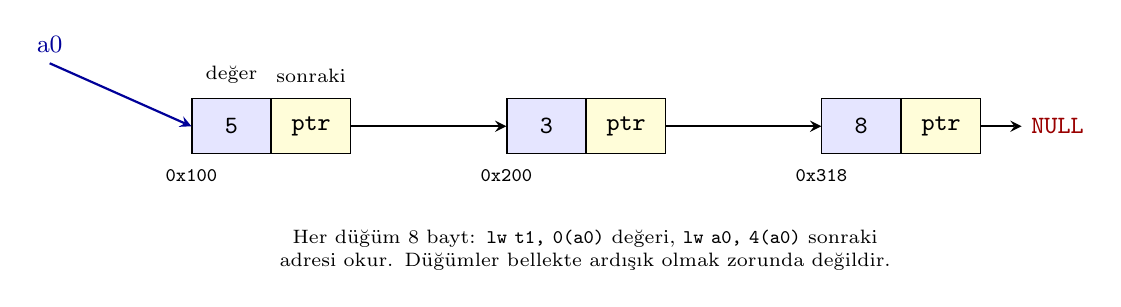
\begin{tikzpicture}[
    node/.style={draw, minimum width=2cm, minimum height=1.4cm, font=\small},
    field/.style={draw, minimum width=1cm, minimum height=0.7cm, font=\small\ttfamily, anchor=west},
    ptr/.style={->, thick, >=stealth},
    null/.style={font=\small\ttfamily, red!60!black}
]
% Node 1
\node[field, fill=blue!10] (v1) at (0,0) {5};
\node[field, fill=yellow!15, anchor=west] (p1) at (v1.east) {ptr};
\node[font=\scriptsize, above=2pt] at (v1.north) {değer};
\node[font=\scriptsize, above=2pt] at (p1.north) {sonraki};
\node[font=\scriptsize\ttfamily, below=2pt] at (v1.south west) {0x100};

% Node 2
\node[field, fill=blue!10] (v2) at (4,0) {3};
\node[field, fill=yellow!15, anchor=west] (p2) at (v2.east) {ptr};
\node[font=\scriptsize\ttfamily, below=2pt] at (v2.south west) {0x200};

% Node 3
\node[field, fill=blue!10] (v3) at (8,0) {8};
\node[field, fill=yellow!15, anchor=west] (p3) at (v3.east) {ptr};
\node[font=\scriptsize\ttfamily, below=2pt] at (v3.south west) {0x318};

% NULL
\node[null] (null) at (11,0) {NULL};

% Arrows — kutunun sağından çıkıp kavisli olarak sonraki düğüme ulaşır
\draw[ptr] (p1.east) to[out=0, in=180] (v2.west);
\draw[ptr] (p2.east) to[out=0, in=180] (v3.west);
\draw[ptr] (p3.east) to[out=0, in=180] (null.west);

% Head pointer
\draw[ptr, blue!60!black] (-1.8,0.8) -- (v1.west) node[pos=0, above, font=\small] {a0};

% Memory note
\node[font=\scriptsize, anchor=north, text width=9cm, align=center] at (5,-1.2) {Her düğüm 8 bayt: \texttt{lw t1, 0(a0)} değeri, \texttt{lw a0, 4(a0)} sonraki adresi okur. Düğümler bellekte ardışık olmak zorunda değildir.};
\end{tikzpicture}
\caption[Bağlı liste veri yapısının bellek görünümü]{Bağlı liste veri yapısının bellek görünümü. Her düğüm bir değer ve sonraki düğümün adresini içerir; son düğümün işaretçisi sıfırdır.}
\label{fig:bagli-liste}
\end{figure}

\begin{bilginot}[Yığın ve Yığıt: İki Farklı Kavram]
Türkçede ``yığın'' sözcüğü hem \emph{heap} (dinamik bellek havuzu) hem de \emph{stack} (yığıt) için kullanılabilir. Bu kitapta karışıklığı önlemek için \emph{stack} karşılığı olarak ``yığıt'', \emph{heap} karşılığı olarak ``yığın'' kullanılmaktadır. Bağlı liste düğümleri uygulamada genellikle yığın (\emph{heap}) üzerinde dinamik olarak oluşturulur.
\end{bilginot}


\subsection{Özyineleme}
\label{subsec:ozyineleme}
\index{özyineleme}\index{recursion|see{özyineleme}}

Önceki örneklerdeki tüm fonksiyonlar yinelemeli (\emph{iterative}) idi: döngüler kullanarak çalışıyorlardı. Ancak bazı problemler, fonksiyonun kendisini çağırmasıyla daha doğal biçimde ifade edilebilir. Bu tekniğe \emph{özyineleme} (\emph{recursion}) denir. Bölüm~\ref{chap:buyruk-kumesi}'te yığıt çerçevesinin nasıl oluşturulduğunu gördük; özyinelemede her çağrı yeni bir yığıt çerçevesi oluşturur. Bu nedenle özyinelemeli fonksiyonlar, yığıt yönetimini anlamak için ideal bir çalışma alanıdır.

\begin{ornek}[4.14]
\label{orn:fibonacci}
$n$'inci Fibonacci sayısını özyinelemeli olarak hesaplayan bir RISC-V fonksiyonu yazın. $F(0) = 0$, $F(1) = 1$, $F(n) = F(n-1) + F(n-2)$.

\textbf{Çözüm:} Önce C dilindeki karşılığı:

\begin{lstlisting}[language=C, style=alistirma-kod]
int fibonacci(int n) {
    if (n <= 1) return n;
    return fibonacci(n - 1) + fibonacci(n - 2);
}
\end{lstlisting}

RISC-V çevirici dilinde (\texttt{a0} = $n$, dönüş değeri \texttt{a0}'da):

\begin{lstlisting}[style=riscv]
# fibonacci: a0 = n
# Dönüş: a0 = F(n)
fibonacci:
    # Taban durumu: n <= 1 ise n döndür
    li   t0, 1
    ble  a0, t0, fib_taban

    # Yığıt çerçevesi: ra, s0, s1 sakla
    addi sp, sp, -12
    sw   ra, 8(sp)
    sw   s0, 4(sp)
    sw   s1, 0(sp)

    mv   s0, a0               # s0 = n
    addi a0, s0, -1           # a0 = n - 1
    jal  fibonacci             # F(n-1) hesapla
    mv   s1, a0               # s1 = F(n-1)

    addi a0, s0, -2           # a0 = n - 2
    jal  fibonacci             # F(n-2) hesapla
    add  a0, s1, a0           # a0 = F(n-1) + F(n-2)

    # Yığıt çerçevesini geri yükle
    lw   s1, 0(sp)
    lw   s0, 4(sp)
    lw   ra, 8(sp)
    addi sp, sp, 12
    ret

fib_taban:
    ret                        # a0 zaten n (0 veya 1)
\end{lstlisting}

Bu programda dikkat edilmesi gereken noktalar:
\begin{itemize}
\item Her özyinelemeli çağrı öncesinde \texttt{ra}, \texttt{s0} ve \texttt{s1} yığıtta saklanır. Saklanan yazmaçlar (\texttt{s0}--\texttt{s11}) çağrılan tarafın sorumluluğundadır; fonksiyon bu yazmaçları bozmamalıdır.
\item İlk \texttt{jal fibonacci} çağrısı \texttt{a0}'daki sonucu döndürür. Bu sonuç \texttt{s1}'e kopyalanır çünkü ikinci çağrı \texttt{a0}'yı değiştirecektir.
\item Taban durumunda yığıt çerçevesi oluşturulmaz; bu, gereksiz bellek erişimini önler.
\item $n = 5$ için bu fonksiyon kendini 15 kez çağırır ve yığıtta en fazla 5 çerçeve (60 bayt) birikir. $n$ büyüdükçe çağrı sayısı üstel olarak artar; bu nedenle büyük $n$ değerleri için yinelemeli sürüm tercih edilmelidir.
\end{itemize}

\emph{Başarım çözümlemesi:} Her özyinelemeli çağrıda 16 buyruk yürütülür: 4 yığıta yazma (\texttt{sw} $\times 3$ + \texttt{addi}), 4 yığıttan okuma (\texttt{lw} $\times 3$ + \texttt{addi}), 2 fonksiyon çağrısı (\texttt{jal}), ve 6 yazmaç işlemi. $n = 5$ için toplam 15 çağrı $\times$ 16 buyruk $= 240$ buyruk yürütülür; bellek buyrukları 2 çevrim alırsa toplam $\sim$336 çevrim, BBÇ $\approx 1{,}40$. Asıl sorun BBÇ değil, buyruk sayısının üstel artışıdır: $n = 10$ için $\sim$177 çağrı $\approx 2832$ buyruk, $n = 20$ için $\sim$21.891 çağrı $\approx 350.000$ buyruk. Yinelemeli sürüm ise $n = 20$ için yalnızca $\sim$120 buyrukla aynı sonucu verir; algoritma seçimi, BBÇ'den çok daha büyük bir başarım etkisi yaratır.
\end{ornek}

\begin{figure}[H]
\centering
\resizebox{0.75\textwidth}{!}{%
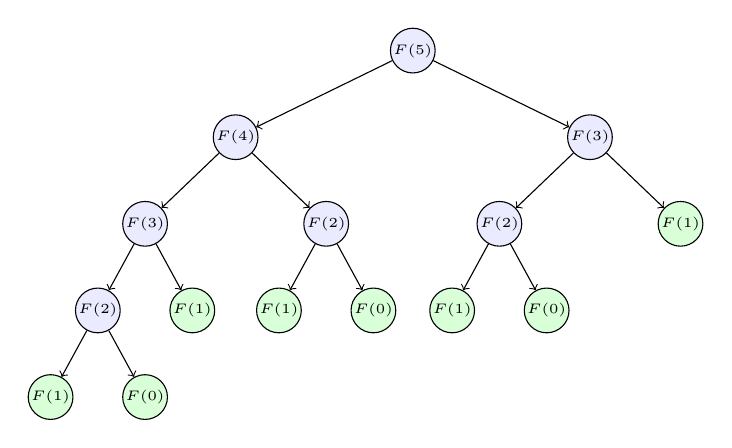
\begin{tikzpicture}[
    level distance=1.1cm,
    every node/.style={draw, circle, minimum size=0.5cm, font=\tiny, fill=blue!8, inner sep=0.5pt},
    edge from parent/.style={draw, ->, thin},
    level 1/.style={sibling distance=4.5cm},
    level 2/.style={sibling distance=2.3cm},
    level 3/.style={sibling distance=1.2cm}
]
\node {$F(5)$}
    child {node {$F(4)$}
        child {node {$F(3)$}
            child {node {$F(2)$}
                child {node[fill=green!15] {$F(1)$}}
                child {node[fill=green!15] {$F(0)$}}
            }
            child {node[fill=green!15] {$F(1)$}}
        }
        child {node {$F(2)$}
            child {node[fill=green!15] {$F(1)$}}
            child {node[fill=green!15] {$F(0)$}}
        }
    }
    child {node {$F(3)$}
        child {node {$F(2)$}
            child {node[fill=green!15] {$F(1)$}}
            child {node[fill=green!15] {$F(0)$}}
        }
        child {node[fill=green!15] {$F(1)$}}
    };
\end{tikzpicture}%
}
\caption[Özyinelemeli Fibonacci çağrı ağacı]{Özyinelemeli Fibonacci çağrı ağacı ($n=5$). Yeşil düğümler taban durumlarıdır; toplam 15 çağrı üretilir ve her çağrı yığıtta 12 baytlık bir çerçeve oluşturur.}
\label{fig:fibonacci-agac}
\end{figure}

\begin{figure}[H]
\centering
\begin{tikzpicture}[scale=0.85]
  \pgfmathsetmacro{\cw}{2.8}
  \pgfmathsetmacro{\ch}{0.55}
  \pgfmathsetmacro{\gap}{0.6}
  \pgfmathsetmacro{\xb}{\cw+\gap+0.7}
  \pgfmathsetmacro{\xc}{2*(\cw+\gap+0.7)}
  \pgfmathsetmacro{\xd}{3*(\cw+\gap+0.7)}
  % Yığıt tepesi yukarıda, yeni çerçeveler üste eklenir
  % Alt kutular ilk çağrılar (yüksek adres), üst kutular son çağrılar (düşük adres)

  % ---- Aşama 1: fib(4) çağrıldı ----
  \node[font=\scriptsize\bfseries] at (\cw/2, 1*\ch+0.35) {(a) fib(4)};
  \draw[thick, fill=blokmavi-acik] (0, 0) rectangle (\cw, 1*\ch);
  \node[font=\tiny] at (\cw/2, 0.5*\ch) {ra, s0=4, s1};
  \draw[okstil, thick, sinyalkirmizi] (\cw+0.5, 1*\ch) -- (\cw, 1*\ch);
  \node[font=\tiny\bfseries, text=sinyalkirmizi, anchor=west] at (\cw+0.55, 1*\ch) {SP};
  \node[font=\tiny, text=gray] at (\cw/2, -0.3*\ch) {12 bayt};

  % ---- Aşama 2: fib(4) → fib(3) ----
  \node[font=\scriptsize\bfseries] at (\xb+\cw/2, 2*\ch+0.35) {(b) fib(3)};
  \draw[thick, fill=blokgri-acik] (\xb, 0) rectangle (\xb+\cw, 1*\ch);
  \node[font=\tiny, text=gray] at (\xb+\cw/2, 0.5*\ch) {fib(4): ra, s0, s1};
  \draw[thick, fill=blokmavi-acik] (\xb, 1*\ch) rectangle (\xb+\cw, 2*\ch);
  \node[font=\tiny] at (\xb+\cw/2, 1.5*\ch) {ra, s0=3, s1};
  \draw[okstil, thick, sinyalkirmizi] (\xb+\cw+0.5, 2*\ch) -- (\xb+\cw, 2*\ch);
  \node[font=\tiny\bfseries, text=sinyalkirmizi, anchor=west] at (\xb+\cw+0.55, 2*\ch) {SP};
  \node[font=\tiny, text=gray] at (\xb+\cw/2, -0.3*\ch) {24 bayt};

  % ---- Aşama 3: fib(4) → fib(3) → fib(2) ----
  \node[font=\scriptsize\bfseries] at (\xc+\cw/2, 3*\ch+0.35) {(c) fib(2)};
  \draw[thick, fill=blokgri-acik] (\xc, 0) rectangle (\xc+\cw, 1*\ch);
  \node[font=\tiny, text=gray] at (\xc+\cw/2, 0.5*\ch) {fib(4): ra, s0, s1};
  \draw[thick, fill=blokgri-acik] (\xc, 1*\ch) rectangle (\xc+\cw, 2*\ch);
  \node[font=\tiny, text=gray] at (\xc+\cw/2, 1.5*\ch) {fib(3): ra, s0, s1};
  \draw[thick, fill=blokmavi-acik] (\xc, 2*\ch) rectangle (\xc+\cw, 3*\ch);
  \node[font=\tiny] at (\xc+\cw/2, 2.5*\ch) {ra, s0=2, s1};
  \draw[okstil, thick, sinyalkirmizi] (\xc+\cw+0.5, 3*\ch) -- (\xc+\cw, 3*\ch);
  \node[font=\tiny\bfseries, text=sinyalkirmizi, anchor=west] at (\xc+\cw+0.55, 3*\ch) {SP};
  \node[font=\tiny, text=gray] at (\xc+\cw/2, -0.3*\ch) {36 bayt};

  % ---- Aşama 4: en derin nokta fib(1) — taban durumu ----
  \node[font=\scriptsize\bfseries] at (\xd+\cw/2, 4*\ch+0.35) {(d) fib(1)};
  \draw[thick, fill=blokgri-acik] (\xd, 0) rectangle (\xd+\cw, 1*\ch);
  \node[font=\tiny, text=gray] at (\xd+\cw/2, 0.5*\ch) {fib(4): ra, s0, s1};
  \draw[thick, fill=blokgri-acik] (\xd, 1*\ch) rectangle (\xd+\cw, 2*\ch);
  \node[font=\tiny, text=gray] at (\xd+\cw/2, 1.5*\ch) {fib(3): ra, s0, s1};
  \draw[thick, fill=blokgri-acik] (\xd, 2*\ch) rectangle (\xd+\cw, 3*\ch);
  \node[font=\tiny, text=gray] at (\xd+\cw/2, 2.5*\ch) {fib(2): ra, s0, s1};
  \draw[thick, fill=blokyesil] (\xd, 3*\ch) rectangle (\xd+\cw, 4*\ch);
  \node[font=\tiny] at (\xd+\cw/2, 3.5*\ch) {fib(1): taban $\rightarrow$ dön};
  \draw[okstil, thick, sinyalkirmizi] (\xd+\cw+0.5, 4*\ch) -- (\xd+\cw, 4*\ch);
  \node[font=\tiny\bfseries, text=sinyalkirmizi, anchor=west] at (\xd+\cw+0.55, 4*\ch) {SP};
  \node[font=\tiny, text=gray] at (\xd+\cw/2, -0.3*\ch) {36 + 0 bayt};

  % ---- Sol kenar: adres yönü ve yığıt tepesi ----
  \draw[->, thick, gray] (-1.5, 3.5*\ch) -- (-1.5, 0.5*\ch)
        node[midway, left, font=\scriptsize, text=gray, align=center] {Adres\\artışı};
  \node[font=\scriptsize, text=gray, anchor=east] at (-1.2, 4.2*\ch) {Düşük adres};
  \node[font=\scriptsize, text=gray, anchor=east] at (-1.2, -0.3*\ch) {Yüksek adres};
  \draw[okstil, thick] (-0.3, 0) -- (-0.3, 4*\ch)
        node[above, font=\scriptsize, align=center] {Yığıt\\tepesi};
\end{tikzpicture}
\caption[Özyinelemeli Fibonacci yığıt büyümesi]{Özyinelemeli Fibonacci çağrısında yığıt çerçevelerinin birikmesi ($n=4$). Her özyinelemeli çağrı yığıtın tepesine 12 baytlık bir çerçeve (ra, s0, s1) ekler. En derin noktada (d) üç çerçeve birikmiştir; taban durumu (fib(1)) çerçeve oluşturmadan döner. Yığıt derinliği $n-1$'e ulaşır.}
\label{fig:fibonacci-yigit-buyumesi}
\end{figure}

\begin{bilginot}[Kuyruk Özyineleme Eniyilemesi]
Bir fonksiyonun son işlemi özyinelemeli çağrı ise buna \emph{kuyruk özyineleme} (\emph{tail recursion}) denir. Derleyici bu durumu algıladığında özyinelemeyi döngüye dönüştürebilir ve yığıt çerçevesi oluşturma gereğini ortadan kaldırır. Yukarıdaki Fibonacci fonksiyonu kuyruk özyinelemeli \emph{değildir} çünkü son işlem \texttt{add} (toplama) buyruğudur, çağrı değil. Ancak bir biriktirici parametresi eklenerek kuyruk özyinelemeli biçime dönüştürülebilir.
\end{bilginot}


\subsection{Çok Fonksiyonlu Programlar}
\label{subsec:cok-fonksiyonlu}
\index{çok fonksiyonlu program}

Fibonacci örneğinde bir fonksiyonun kendisini çağırdığını gördük. Gerçek programlarda ise farklı fonksiyonlar birbirini çağırarak bir iş akışı oluşturur. Bu durumda Örnek~4.6'da öğrendiğimiz yaprak/yaprak olmayan ayrımı kritik hale gelir: hangi fonksiyon \texttt{ra}'yı saklamalı, hangi yazmaçlar korunmalı? Şimdi bu soruları somut bir örnekle yanıtlayalım.

\begin{ornek}[4.15]
\label{orn:cok-fonksiyon}
Bellekteki bir dizinin en büyük ve en küçük elemanını bulan, ardından bunların farkını hesaplayan bir program yazın. Program üç fonksiyondan oluşsun: \texttt{en\_buyuk}, \texttt{en\_kucuk} ve \texttt{main}.

\textbf{Çözüm:}

\begin{lstlisting}[style=riscv]
.data
dizi:    .word  12, 5, 23, 7, 18, 3, 15
boyut:   .word  7
sonuc:   .word  0

.text
.globl main
main:
    addi sp, sp, -4
    sw   ra, 0(sp)

    la   a0, dizi
    lw   a1, boyut            # a1 = 7
    jal  en_buyuk              # a0 = en büyük
    mv   s0, a0               # s0 = en büyük

    la   a0, dizi
    lw   a1, boyut
    jal  en_kucuk              # a0 = en küçük

    sub  t0, s0, a0           # t0 = en büyük - en küçük
    la   t1, sonuc
    sw   t0, 0(t1)            # sonucu belleğe yaz

    lw   ra, 0(sp)
    addi sp, sp, 4
    li   a7, 10
    ecall

# en\_buyuk: a0=dizi adresi, a1=boyut
# Dönüş: a0 = en büyük eleman
en_buyuk:
    lw   t0, 0(a0)            # t0 = dizi[0] (geçici en büyük)
    li   t1, 1                # t1 = i = 1
eb_dongu:
    bge  t1, a1, eb_son
    slli t2, t1, 2
    add  t2, a0, t2
    lw   t3, 0(t2)            # t3 = dizi[i]
    ble  t3, t0, eb_atla      # dizi[i] <= en büyük ise atla
    mv   t0, t3               # yeni en büyük
eb_atla:
    addi t1, t1, 1
    j    eb_dongu
eb_son:
    mv   a0, t0
    ret

# en\_kucuk: a0=dizi adresi, a1=boyut
# Dönüş: a0 = en küçük eleman
en_kucuk:
    lw   t0, 0(a0)            # t0 = dizi[0] (geçici en küçük)
    li   t1, 1                # t1 = i = 1
ek_dongu:
    bge  t1, a1, ek_son
    slli t2, t1, 2
    add  t2, a0, t2
    lw   t3, 0(t2)            # t3 = dizi[i]
    bge  t3, t0, ek_atla      # dizi[i] >= en küçük ise atla
    mv   t0, t3               # yeni en küçük
ek_atla:
    addi t1, t1, 1
    j    ek_dongu
ek_son:
    mv   a0, t0
    ret
\end{lstlisting}

Bu programda \texttt{main} fonksiyonu sırasıyla \texttt{en\_buyuk} ve \texttt{en\_kucuk} fonksiyonlarını çağırır. Dikkat edilmesi gereken noktalar:
\begin{itemize}
\item \texttt{main} fonksiyonu başka fonksiyonları çağırdığı için \texttt{ra}'yı yığıtta saklar. Eğer \texttt{main} yaprak fonksiyon olsaydı (başka fonksiyon çağırmayan) bu gerekli olmazdı.
\item \texttt{en\_buyuk} fonksiyonunun sonucu \texttt{s0}'a kopyalanır. Bu bir saklanan yazmaç olduğu için \texttt{en\_kucuk} çağrısı sırasında korunacaktır. Geçici yazmaç (\texttt{t0}--\texttt{t6}) kullanılsaydı, \texttt{en\_kucuk} fonksiyonu bu değeri bozabilirdi.
\item Her iki alt fonksiyon yalnızca geçici yazmaçlar kullandığı ve başka fonksiyon çağırmadığı için (yaprak fonksiyonlar) yığıt çerçevesi oluşturmazlar.
\end{itemize}

\emph{Başarım çözümlemesi:} Bu programda \texttt{main} 12 buyruk, \texttt{en\_buyuk} ve \texttt{en\_kucuk} ise her biri $6n + 2$ buyruk yürütür ($n$ = dizi boyutu). $n = 7$ için toplam: $12 + 2 \times (6 \times 7 + 2) = 100$ buyruk. Her döngü gövdesinde 1 bellek erişimi (\texttt{lw}) ve 1 dallanma vardır; \texttt{main}'de ise 2 bellek erişimi (\texttt{sw}/\texttt{lw} yığıt) bulunur. Bellek buyrukları 2 çevrim alırsa: yazmaç buyrukları $\sim$72, bellek buyrukları $\sim$16, dallanma buyrukları $\sim$12 ile toplam $72 + 32 + 24 = 128$ çevrim, BBÇ $\approx 1{,}28$. Dikkat edilmesi gereken bir nokta: yaprak fonksiyonlarda yığıt çerçevesi oluşturulmadığı için bellek erişimi azalır ve BBÇ düşer. Yaprak olmayan \texttt{main} ise \texttt{ra} saklama/yükleme nedeniyle fazladan 2 bellek erişimi gerektirir.
\end{ornek}


\begin{tanim}[Tasarım İlkesi 3: Olağan durumu hızlandır \emph{(devam)}]
Derleyicilerin uyguladığı eniyilemeler bu ilkenin doğrudan yansımasıdır: en sık yürütülen kod yolları (döngü gövdeleri, sık çağrılan fonksiyonlar) için daha az buyruk üreten ve daha az bellek erişimi gerektiren kod üretilir. Programcı da aynı ilkeyi çevirici dil düzeyinde uygulayabilir: seyrek çalışan hata kontrolü kodunu döngü dışına taşımak, sık erişilen verileri yazmaçlarda tutmak gibi.
\end{tanim}

% =====================================================
\section{C'den RISC-V'e: Derleme Çıktısı Okuma}
\label{sec:derleme-ciktisi}
\index{derleyici çıktısı}\index{derleme}

Bir bilgisayar mimarı ya da sistem programcısı için en değerli becerilerden biri, derleyicinin ürettiği çevirici dil kodunu okuyabilmektir. Bu bölümde, GCC derleyicisinin C kodundan ürettiği RISC-V çevirici dil çıktısını inceleyeceğiz.

\subsection{Derleyici Çıktısı Elde Etme}
\label{subsec:derleyici-ciktisi}

GCC ile RISC-V çevirici dil çıktısı almak için \texttt{-S} seçeneği kullanılır:

\begin{lstlisting}[language=bash]
riscv64-unknown-elf-gcc -S -O0 -march=rv32i -mabi=ilp32 program.c
\end{lstlisting}

Bu komut, \texttt{program.s} dosyasını üretir. \texttt{-O0} eniyileme yapılmadığını, \texttt{-march=rv32i} hedef mimarinin RV32I olduğunu belirtir.

\subsection{Eniyileme Seviyelerinin Etkisi}
\label{subsec:eniyileme}
\index{eniyileme}\index{optimization|see{eniyileme}}

Derleyicinin eniyileme seviyesi, üretilen kodun yapısını köklü biçimde değiştirir. Aşağıdaki basit fonksiyonu farklı seviyelerde derleyerek farkları görelim:

\begin{ornek}[4.16]
\label{orn:eniyileme}
Aşağıdaki C fonksiyonunun \texttt{-O0} ve \texttt{-O2} ile derlenen çıktılarını karşılaştırın:

\begin{lstlisting}[language=C, style=alistirma-kod]
int toplam(int dizi[], int n) {
    int sonuc = 0;
    for (int i = 0; i < n; i++)
        sonuc += dizi[i];
    return sonuc;
}
\end{lstlisting}

\textbf{Çözüm:} \texttt{-O0} (eniyileme yok) çıktısı; derleyici her değişkeni yığıtta saklar:

\begin{lstlisting}[style=riscv]
# -O0: Her değişken yığıtta, her erişimde lw/sw
toplam:
    addi sp, sp, -32
    sw   ra, 28(sp)
    sw   s0, 24(sp)
    addi s0, sp, 32           # çerçeve işaretçisi
    sw   a0, -20(s0)          # dizi adresini yığıtta sakla
    sw   a1, -24(s0)          # n'i yığıtta sakla
    sw   zero, -28(s0)        # sonuc = 0
    sw   zero, -32(s0)        # i = 0
    j    dongu_kontrol
dongu_govde:
    lw   t0, -32(s0)          # i'yi yığıttan oku
    slli t0, t0, 2
    lw   t1, -20(s0)          # dizi adresini yığıttan oku
    add  t0, t1, t0
    lw   t0, 0(t0)            # dizi[i]
    lw   t1, -28(s0)          # sonuc'u yığıttan oku
    add  t1, t1, t0
    sw   t1, -28(s0)          # sonuc'u yığıta yaz
    lw   t0, -32(s0)          # i'yi yığıttan oku
    addi t0, t0, 1
    sw   t0, -32(s0)          # i'yi yığıta yaz
dongu_kontrol:
    lw   t0, -32(s0)          # i'yi yığıttan oku
    lw   t1, -24(s0)          # n'i yığıttan oku
    blt  t0, t1, dongu_govde
    lw   a0, -28(s0)          # dönüş değeri = sonuc
    lw   s0, 24(sp)
    lw   ra, 28(sp)
    addi sp, sp, 32
    ret
\end{lstlisting}

\texttt{-O2} (eniyileme açık) çıktısı; derleyici değişkenleri yazmaçlarda tutar:

\begin{lstlisting}[style=riscv]
# -O2: Değişkenler yazmaçlarda, gereksiz erişim yok
toplam:
    li   a5, 0                # sonuc = 0
    ble  a1, zero, son        # n <= 0 ise hemen dön
    slli a1, a1, 2            # a1 = n * 4
    add  a1, a0, a1           # a1 = \&dizi[n] (bitiş adresi)
dongu:
    lw   a4, 0(a0)            # a4 = dizi[i]
    addi a0, a0, 4            # işaretçiyi ilerlet
    add  a5, a5, a4           # sonuc += dizi[i]
    bne  a0, a1, dongu        # bitiş adresine ulaşmadıysa devam
son:
    mv   a0, a5               # dönüş değeri = sonuc
    ret
\end{lstlisting}

\texttt{-O2} çıktısında dikkat çeken farklar:
\begin{itemize}
\item Yığıt çerçevesi oluşturulmamıştır; tüm değişkenler yazmaçlarda tutulur.
\item Döngü sayacı (\texttt{i}) yerine işaretçi kullanılır; bu, her yinelemede \texttt{slli} ile çarpma yapma gereğini ortadan kaldırır.
\item Döngü gövdesinde yalnızca 4 buyruk vardır (\texttt{-O0}'da 10'dan fazla).
\item Döngü kontrolü sona alınmıştır (\emph{loop inversion}): döngü başında bir defa kontrol yapılır, sonra gövde-kontrol sırası tersine çevrilir.
\end{itemize}
\end{ornek}

\begin{bilginot}[Derleyiciye Güvenmek]
Çağdaş derleyiciler çoğu durumda insandan daha iyi çevirici dil kodu üretir. Elle çevirici dil yazmanın anlamlı olduğu durumlar sınırlıdır: önyükleme kodu, kesme işleyicileri, çok hassas zamanlama gerektiren gömülü sistemler ve kriptografi gibi alanlarda elle yazılmış kod gerekebilir. Derleyici çıktısını okumak, çevirici dilde programlamaktan çok daha yaygın ve değerli bir beceridir. Derleyicinin ürettiği kodun boru hattıyla nasıl etkileşime girdiğini (dallanma gecikmesi yuvası, yük kullanım gecikmesi gibi kavramları) Bölüm~\ref{chap:boruhatti}'de ele alacağız.
\end{bilginot}


\subsection{Yapısal Dönüşümler}
\label{subsec:yapisal-donusumler}
\index{derleyici!eniyileme}

Derleyicilerin uyguladığı bazı yaygın dönüşümler şunlardır:

\begin{table}[H]
\centering
\caption[Yaygın derleyici eniyilemeleri]{Yaygın derleyici eniyilemeleri}
\label{tab:derleyici-eniyilemeleri}
\small
\begin{tabularx}{\textwidth}{l X X}
\toprule
\textbf{Eniyileme} & \textbf{C Düzeyinde} & \textbf{Etki} \\
\midrule
Sabit katlama & \texttt{x = 3 * 4} $\rightarrow$ \texttt{x = 12} & Derleme zamanında hesaplama \\
Güç azaltma & \texttt{x * 4} $\rightarrow$ \texttt{x << 2} & Çarpma yerine kaydırma \\
Döngü değişmezi taşıma & Döngüde değişmeyen hesabı dışarı çıkarma & Daha az buyruk yürütme \\
Ölü kod eleme & Kullanılmayan değişkenleri silme & Daha az buyruk \\
Döngü açma & \texttt{for} gövdesini $k$ kez tekrarlama & Dallanma sayısını azaltma \\
Kuyruk çağrısı eleme & Özyinelemeli çağrıyı döngüye çevirme & Yığıt taşmasını önleme \\
\bottomrule
\end{tabularx}
\end{table}

\begin{karsilastirma}[Derleyici Çıktısı: RISC-V, ARM ve x86]
Aynı C fonksiyonunun farklı mimarilerde derlenmiş çıktıları, BKM tasarım kararlarının etkisini somut biçimde gösterir.

\emph{RISC-V:} Sabit 32 bitlik buyruklar, yükle/sakla mimarisi. Döngü gövdesi genellikle 4--6 buyruktan oluşur. Yazmaç adları açık ve tutarlıdır (\texttt{a0}, \texttt{t0}, \texttt{s0}).

\emph{ARM AArch64:} RISC-V'e çok benzer yapıda (sabit 32 bit buyruk, yükle/sakla). Koşullu yürütme ve bayt ters çevirme gibi ek buyruklar daha yoğun kod üretebilir. Derleyici çıktısında \texttt{ldr}/\texttt{str} ve \texttt{x0}--\texttt{x30} yazmaçları kullanılır.

\emph{x86-64:} Değişken uzunluklu buyruklar (1--15 bayt). Bellek-yazmaç buyrukları sayesinde ayrı yükleme buyruğu gerekmez: \texttt{add eax, [rdi]} tek buyrukla hem bellek okur hem toplar. Ancak bu karmaşıklık çözücü donanımını büyütür.

Her üç mimaride de \texttt{-O2} seviyesinde döngü gövdeleri birbirine oldukça yakın buyruk sayısına sahiptir; asıl fark buyruk kodlama boyutunda ve çözücü karmaşıklığında ortaya çıkar.
\end{karsilastirma}

\begin{ornek}[4.17]
\label{orn:guc-azaltma}
Güç azaltma (\emph{strength reduction}) eniyilemesini bir örnekle gösterin.

\textbf{Çözüm:} Aşağıdaki C kodunda dizi erişimi her yinelemede çarpma gerektirir:

\begin{lstlisting}[language=C, style=alistirma-kod]
for (int i = 0; i < n; i++)
    dizi[i] = 0;              // adres = dizi + i * 4
\end{lstlisting}

Eniyileme öncesi her yinelemede \texttt{slli} + \texttt{add} ile adres hesaplanır. Eniyileme sonrası derleyici bunu işaretçi artırımına dönüştürür:

\begin{lstlisting}[style=riscv]
# Eniyileme öncesi (her yinelemede i*4 hesapla)
    li   t0, 0                # i = 0
dongu1:
    bge  t0, a1, son1
    slli t1, t0, 2            # t1 = i * 4
    add  t1, a0, t1           # t1 = \&dizi[i]
    sw   zero, 0(t1)          # dizi[i] = 0
    addi t0, t0, 1
    j    dongu1
son1:

# Eniyileme sonrası (işaretçi artır)
    slli t0, a1, 2            # t0 = n * 4
    add  t0, a0, t0           # t0 = bitiş adresi
    mv   t1, a0               # t1 = geçerli adres
dongu2:
    bge  t1, t0, son2
    sw   zero, 0(t1)          # *p = 0
    addi t1, t1, 4            # p += 4
    j    dongu2
son2:
\end{lstlisting}

İkinci sürümde döngü gövdesinde çarpma yoktur; yalnızca bir \texttt{sw} ve bir \texttt{addi} vardır.
\end{ornek}


% =====================================================
\section{Gömülü Sistem Programlama}
\label{sec:gomulu-sistem}
\index{gömülü sistem}\index{embedded system|see{gömülü sistem}}

RISC-V mimarisi gömülü sistemlerde giderek yaygınlaşmaktadır. Bu bölümde, işletim sistemi olmadan çalışan (\emph{bare-metal}) programlama ve bellek eşlemeli giriş/çıkış (MMIO) kavramlarını ele alacağız.

\subsection{Bellek Eşlemeli Giriş/Çıkış}
\label{subsec:mmio}
\index{bellek eşlemeli giriş/çıkış}\index{MMIO|see{bellek eşlemeli giriş/çıkış}}

Gömülü sistemlerde çevresel aygıtlar (LED, düğme, UART, zamanlayıcı) bellek adres uzayının belirli bölgelerine eşlenir. Bu adreslere yazma ve okuma işlemleri, doğrudan donanımla iletişim kurar. Bu yönteme bellek eşlemeli giriş/çıkış (\emph{Memory-Mapped I/O}, MMIO) denir.

\begin{ornek}[4.18]
\label{orn:mmio-led}
Bellek adresine eşlenmiş bir LED'i yakıp söndüren bir RISC-V programı yazın. LED kontrol yazmacı \texttt{0x10012008} adresinde olsun ve 0. bit LED'in durumunu kontrol etsin.

\textbf{Çözüm:}

\begin{lstlisting}[style=riscv]
.equ LED_ADDR, 0x10012008    # LED kontrol yazmacı adresi

.text
.globl main
main:
    li   t0, LED_ADDR         # LED yazmacı adresi
    li   t1, 1                # bit 0 = 1 (LED yak)
    sw   t1, 0(t0)            # LED'i yak

    # Basit gecikme döngüsü
    li   t2, 1000000
gecikme:
    addi t2, t2, -1
    bnez t2, gecikme

    sw   zero, 0(t0)          # LED'i söndür
    j    main                 # başa dön (sürekli yanıp sön)
\end{lstlisting}

Bu programda \texttt{sw t1, 0(t0)} buyruğu sıradan bir bellek yazma gibi görünür, ancak hedef adres bir donanım yazmacına eşlendiği için yazılan değer doğrudan LED'in durumunu değiştirir. Bu, RISC-V'in (ve genel olarak RISC mimarilerinin) giriş/çıkış felsefesini yansıtır: ayrı giriş/çıkış buyrukları yerine standart bellek erişim buyrukları kullanılır.
\end{ornek}

\begin{bilginot}[Uçucu Bellek Erişimi ve Derleyici]
Bellek eşlemeli giriş/çıkış adreslerine yapılan erişimlerde derleyicinin eniyileme yapması tehlikeli olabilir. Derleyici, aynı adrese yapılan ardışık okuma işlemlerini gereksiz sayarak birini eleyebilir; ancak donanım yazmacının değeri her okumada farklı olabilir (örneğin durum yazmacı). C dilinde bu sorunu önlemek için \texttt{volatile} niteleyicisi kullanılır. Çevirici dilde ise tüm bellek erişimleri açık biçimde yazıldığı için bu sorun oluşmaz; ancak derleyici çıktısını okurken \texttt{volatile} erişimlerinin elenmediğini doğrulamak önemlidir.
\end{bilginot}

\subsection{UART ile Seri İletişim}
\label{subsec:uart}
\index{UART}

UART (\emph{Universal Asynchronous Receiver/Transmitter}), gömülü sistemlerde en yaygın seri iletişim arabirimidir. RISC-V tabanlı mikrodenetleyicilerde UART da MMIO ile erişilir.

\begin{ornek}[4.19]
\label{orn:uart}
UART üzerinden bir karakter dizisi gönderen bir RISC-V programı yazın. UART veri yazmacı \texttt{0x10013000} adresinde, durum yazmacı \texttt{0x10013004} adresinde olsun. Durum yazmacının 0.\ biti ``gönderme hazır'' bayrağıdır.

\textbf{Çözüm:}

\begin{lstlisting}[style=riscv]
.equ UART_TX,     0x10013000  # UART veri yazmacı
.equ UART_STATUS, 0x10013004  # UART durum yazmacı

.data
ileti: .asciz "Merhaba RISC-V!\n"

.text
.globl main
main:
    la   a0, ileti            # ileti adresini yükle
    jal  uart_yazdir          # yazdırma fonksiyonunu çağır
    j    main                 # sürekli tekrarla

# uart\_yazdir: a0 = karakter dizisi adresi
uart_yazdir:
    li   t0, UART_TX
    li   t1, UART_STATUS
yazdir_dongu:
    lb   t2, 0(a0)            # bir karakter oku
    beqz t2, yazdir_son       # sıfır karakterse bitir
bekle:
    lw   t3, 0(t1)            # durum yazmacını oku
    andi t3, t3, 1            # hazır biti kontrol et
    beqz t3, bekle            # hazır değilse bekle
    sw   t2, 0(t0)            # karakteri gönder
    addi a0, a0, 1            # sonraki karakter
    j    yazdir_dongu
yazdir_son:
    ret
\end{lstlisting}

Bu programdaki ``meşgul bekleme'' (\emph{busy waiting}) döngüsü (\texttt{bekle} etiketi) gömülü sistemlerde yaygın bir kalıptır. İşlemci, UART'ın önceki karakteri göndermeyi bitirmesini bekler. Daha verimli bir yöntem olarak kesmeler (\emph{interrupts}) kullanılabilir; bu konu Bölüm~\ref{chap:giris-cikis}'da ele alınacaktır.
\end{ornek}


% =====================================================
\section{Başarım ve Eniyileme}
\label{sec:basarim-eniyileme}
\index{başarım!çevirici dil}

Çevirici dil düzeyinde programlamanın önemli bir boyutu da başarım çözümlemesidir. Bu bölümde bir programın kaç buyruk yürüttüğünü saymayı ve döngü eniyilemelerinin etkisini inceleyeceğiz.

\subsection{Buyruk Sayımı ve Döngü Gövdesi Çözümlemesi}
\label{subsec:buyruk-sayimi}
\index{buyruk sayımı}

Bir programın yürütme süresini öngörmenin en basit yolu, toplam yürütülen buyruk sayısını hesaplamaktır. Bölüm~\ref{chap:basarim}'de gördüğümüz başarım denklemini hatırlayalım:

\[
\text{Yürütme süresi} = \text{Buyruk sayısı} \times \text{BBÇ} \times \text{Saat dönem süresi}
\]

\begin{ornek}[4.20]
\label{orn:buyruk-sayimi}
Örnek~\ref{orn:dogrusal-arama}'daki doğrusal arama fonksiyonu, $n$ elemanlı bir dizide aranan değerin dizide bulunmadığı en kötü durumda kaç buyruk yürütür?

\textbf{Çözüm:} Döngü gövdesindeki buyrukları sayalım:

\begin{center}
\small
\begin{tabular}{l l c}
\toprule
\textbf{Buyruk} & \textbf{Açıklama} & \textbf{Sayı} \\
\midrule
\texttt{bge t0, a1, bulunamadi} & sınır kontrolü & 1 \\
\texttt{slli t1, t0, 2} & dizin $\rightarrow$ bayt uzaklığı & 1 \\
\texttt{add t1, a0, t1} & adres hesaplama & 1 \\
\texttt{lw t2, 0(t1)} & bellek okuma & 1 \\
\texttt{beq t2, a2, bulundu} & değer karşılaştırma & 1 \\
\texttt{addi t0, t0, 1} & sayaç artırma & 1 \\
\texttt{j dongu} & döngü başına dön & 1 \\
\bottomrule
\end{tabular}
\end{center}

Döngü gövdesi her yinelemede 7 buyruk yürütür. $n$ elemanlı dizide aranan değer bulunamazsa döngü $n$ kez çalışır. Başlangıçtaki \texttt{li} ve sondaki \texttt{li} + \texttt{ret} buyruklarıyla birlikte:

\[
\text{Toplam buyruk} = 1 + 7n + 1 + 1 + 1 = 7n + 4
\]

$n = 1000$ için toplamda 7004 buyruk yürütülür. Eğer BBÇ = 1 ve saat sıklığı 100~MHz ise yürütme süresi yaklaşık $70{,}04~\mu\text{s}$ olur.
\end{ornek}

\subsection{Döngü Açma}
\label{subsec:dongu-acma}
\index{döngü açma}\index{loop unrolling|see{döngü açma}}

Döngü açma (\emph{loop unrolling}), döngü gövdesini birden çok kez tekrarlayarak dallanma buyruğu sayısını azaltan bir eniyileme tekniğidir.

\begin{ornek}[4.21]
\label{orn:dongu-acma}
Aşağıdaki dizi toplama döngüsünü 4 kat açarak (\emph{4-way unroll}) buyruk sayısının nasıl değiştiğini gösterin.

\textbf{Çözüm:} Özgün döngü her yinelemede 1 eleman işler (4 buyruk + 1 dallanma):

\begin{lstlisting}[style=riscv]
# Özgün: her yinelemede 1 eleman
dongu:
    bge  t0, t3, son          # 1 dallanma
    lw   t1, 0(t0)            # 1 bellek okuma
    add  t2, t2, t1           # 1 toplama
    addi t0, t0, 4            # 1 işaretçi artırma
    j    dongu                # 1 dallanma
\end{lstlisting}

4 kat açılmış döngü her yinelemede 4 eleman işler:

\begin{lstlisting}[style=riscv]
# 4 kat açılmış: her yinelemede 4 eleman
dongu_acik:
    bge  t0, t4, kalan        # t4 = bitiş - 16
    lw   t1, 0(t0)            # eleman 1
    lw   t5, 4(t0)            # eleman 2
    lw   t6, 8(t0)            # eleman 3
    lw   a4, 12(t0)           # eleman 4
    add  t2, t2, t1
    add  t2, t2, t5
    add  t2, t2, t6
    add  t2, t2, a4
    addi t0, t0, 16           # işaretçiyi 16 bayt ilerlet
    j    dongu_acik
kalan:                        # kalan elemanları tek tek işle
    bge  t0, t3, son
    lw   t1, 0(t0)
    add  t2, t2, t1
    addi t0, t0, 4
    j    kalan
son:
\end{lstlisting}

Açılmış döngüde her 4 eleman için 11 buyruk yürütülür (2 dallanma + 4 yükleme + 4 toplama + 1 artırma). Özgün döngüde aynı 4 eleman için 20 buyruk gerekir ($5 \times 4$). Bu, yaklaşık \%45 buyruk azalması demektir. Döngü açmanın boru hattı başarımı üzerindeki etkisi Bölüm~\ref{chap:boruhatti}'de ayrıntılı olarak incelenecektir.
\end{ornek}


\subsection{Matris İşlemleri ve Bellek Erişim Kalıpları}
\label{subsec:matris-erişim}
\index{bellek erişim kalıbı}\index{matris çarpımı}

Matris işlemleri, bellek erişim kalıplarının başarım üzerindeki etkisini görmek için ideal bir çalışma alanıdır. C dilinde iki boyutlu diziler satır öncelikli (\emph{row-major}) düzende saklanır: \texttt{A[0][0]}, \texttt{A[0][1]}, \texttt{A[0][2]}, \ldots\ şeklinde ardışık bellek adreslerinde yer alır.

\begin{ornek}[4.22]
\label{orn:matris-toplam}
$4 \times 4$ boyutunda iki matrisin toplamını hesaplayan bir RISC-V programı yazın ve bellek erişim kalıbını çözümleyin.

\textbf{Çözüm:} Matrisler bellekte satır öncelikli düzende, her eleman \texttt{.word} (4 bayt) olarak saklanır. $4 \times 4$ matris $16 \times 4 = 64$ bayt yer kaplar.

\begin{lstlisting}[style=riscv]
# matris\_toplam: a0=A adresi, a1=B adresi, a2=C adresi
# C[i][j] = A[i][j] + B[i][j], 4x4 matris
matris_toplam:
    li   t0, 16               # toplam eleman sayısı
    li   t1, 0                # sayaç = 0
mt_dongu:
    bge  t1, t0, mt_son
    slli t2, t1, 2            # bayt uzaklığı = sayaç * 4
    add  t3, a0, t2           # \&A[i][j]
    add  t4, a1, t2           # \&B[i][j]
    add  t5, a2, t2           # \&C[i][j]
    lw   t3, 0(t3)            # A[i][j]
    lw   t4, 0(t4)            # B[i][j]
    add  t3, t3, t4           # A[i][j] + B[i][j]
    sw   t3, 0(t5)            # C[i][j] = sonuç
    addi t1, t1, 1
    j    mt_dongu
mt_son:
    ret
\end{lstlisting}

Bu programda matris erişimi doğrusal (ardışık) olduğu için bellek erişim kalıbı verimlidir: her yinelemede üç ardışık bellek konumuna erişilir. Matris çarpımında ise durum farklıdır: B matrisinin sütunlarına erişim, her adımda $4 \times 4 = 16$ baytlık sıçramalar gerektirir. Bu düzensiz erişim kalıbı önbellek başarımını olumsuz etkiler; bu konu Bölüm~\ref{chap:bellek}'de ayrıntılı olarak incelenecektir.
\end{ornek}

\begin{bilginot}[Alanda Yerellik ve Zamanda Yerellik]
\index{alanda yerellik}\index{zamanda yerellik}
Bellek erişim kalıplarında iki temel yerellik türü vardır. \emph{Alanda yerellik} (\emph{spatial locality}): bir bellek konumuna erişildiyse yakındaki konumlara da yakında erişilme olasılığı yüksektir; matris satır erişimi buna örnektir. \emph{Zamanda yerellik} (\emph{temporal locality}): bir bellek konumuna erişildiyse aynı konuma yakında tekrar erişilme olasılığı yüksektir; döngü sayacı buna örnektir. Önbellek tasarımı bu iki yerellik türünden faydalanır. Bir programın erişim kalıplarını anlamak, başarım eniyilemesinin ilk adımıdır.
\end{bilginot}


% =====================================================
\section{Hata Ayıklama}
\label{sec:hata-ayiklama}
\index{hata ayıklama}\index{debugging|see{hata ayıklama}}

Çevirici dil programlarında hata ayıklama, yüksek düzeyli dillere kıyasla daha zahmetlidir çünkü derleyicinin sunduğu tür denetimi ve bellek güvenliği gibi korumalar yoktur. Bu bölümde yaygın hataları ve hata ayıklama yöntemlerini ele alacağız.

\subsection{Yaygın Hatalar}
\label{subsec:yaygın-hatalar}

\begin{table}[H]
\centering
\caption[Çevirici dilde sık yapılan hatalar]{Çevirici dilde sık yapılan hatalar}
\label{tab:yaygın-hatalar}
\small
\begin{tabularx}{\textwidth}{l X X}
\toprule
\textbf{Hata Türü} & \textbf{Belirti} & \textbf{Çözüm} \\
\midrule
Yığıt hizalama & \texttt{sp} değeri 4'ün (veya 16'nın) katı değil & \texttt{addi sp, sp, -N} ile N'i doğru hesaplayın \\
\texttt{ra} kaybı & Fonksiyondan dönüşte yanlış adrese atlanma & İç içe çağrılarda \texttt{ra}'yı yığıtta saklayın \\
Bayt/sözcük karışıklığı & Dizi erişiminde yanlış eleman okunması & Dizin $\times$ eleman boyutu unutulmamalı \\
İşaret genişletme & \texttt{lb} ile yüklenen $> 127$ değer negatif olur & İşaretsiz veriler için \texttt{lbu} kullanın \\
Dal uzaklığı & Uzak etikete dallanma başarısız & \texttt{j} veya ters koşul + \texttt{j} birleşimi kullanın \\
Saklanan yazmaç ihlali & Çağrılan fonksiyon \texttt{s0}--\texttt{s11}'i bozar & Kullanılan \texttt{s} yazmaçlarını yığıtta saklayın \\
\bottomrule
\end{tabularx}
\end{table}

\begin{ornek}[4.23]
\label{orn:hata-ornek}
Aşağıdaki programdaki hataları bulun ve düzeltin:

\begin{lstlisting}[style=riscv]
# HATALI KOD: Dizi elemanlarını topla
toplam:
    li   t0, 0                # i = 0
    li   t1, 0                # sonuc = 0
dongu:
    bge  t0, a1, bitti
    add  t2, a0, t0           # HATA 1: bayt uzaklığı yok!
    lw   t3, 0(t2)
    add  t1, t1, t3
    addi t0, t0, 1
    j    dongu
bitti:
    mv   a0, t1
    ret
\end{lstlisting}

\textbf{Çözüm:} Hata 1: \texttt{add t2, a0, t0} satırında dizin doğrudan adrese ekleniyor. Her \texttt{.word} 4 bayt olduğu için dizin önce 4 ile çarpılmalı:

\begin{lstlisting}[style=riscv]
    slli t2, t0, 2            # t2 = i * 4
    add  t2, a0, t2           # t2 = \&dizi[i]
\end{lstlisting}

Bu tür bir hata, programın çökmesine veya yanlış bellek konumlarının okunmasına yol açar. Hatanın belirtisi: sonucun beklenenden çok farklı olması ya da hizalama hatası (\emph{misaligned access}) istisnası.
\end{ornek}

\begin{ornek}[4.24]
\label{orn:hata-ra}
Aşağıdaki programda hata bulun. Program \texttt{kare} fonksiyonunu çağırıp sonucu yazdırmak istiyor; ancak çalıştırıldığında sonsuz döngüye giriyor.

\begin{lstlisting}[style=riscv]
# HATALI KOD: a0'daki sayının karesini yazdır
.text
.globl main
main:
    li   a0, 7
    jal  kare
    # a0 = 49 olmalı
    li   a7, 1
    ecall
    li   a7, 10
    ecall

kare:
    mul  a0, a0, a0
    ret

# hesapla: kareden sonra bir şey daha yap
hesapla:
    li   a0, 5
    jal  kare                  # ra üzerine yazılır!
    # ...
    ret                        # ra artık yanlış adresi gösterir
\end{lstlisting}

\textbf{Çözüm:} \texttt{hesapla} fonksiyonu yaprak olmayan bir fonksiyondur (başka fonksiyon çağırır), ancak \texttt{ra}'yı yığıtta saklamamıştır. \texttt{jal kare} buyruğu \texttt{ra}'nın üzerine yeni bir dönüş adresi yazar ve eski değer kaybolur. \texttt{ret} çalıştığında \texttt{ra} \texttt{kare}'nin çağrıldığı satırın hemen sonrasını gösterir; bu da \texttt{jal kare}'nin tekrar çalışmasına ve sonsuz döngüye yol açar.

Düzeltilmiş sürüm:

\begin{lstlisting}[style=riscv]
hesapla:
    addi sp, sp, -4
    sw   ra, 0(sp)             # ra'yı sakla
    li   a0, 5
    jal  kare
    # ...
    lw   ra, 0(sp)             # ra'yı geri yükle
    addi sp, sp, 4
    ret                        # artık doğru adrese döner
\end{lstlisting}

Bu hata, çevirici dil programlamada en sinsi hatalardan biridir: program çökmez, yalnızca sonsuz döngüye girer. RARS'ta \texttt{ra} yazmacının değerini izleyerek hatanın kaynağını bulmak mümkündür.
\end{ornek}

\subsection{RARS ile Adım Adım Yürütme}
\label{subsec:rars-hata-ayiklama}
\index{RARS!hata ayıklama}

RARS benzetimliği, hata ayıklama için güçlü araçlar sunar:

\begin{itemize}
\item Kesme noktası (\emph{breakpoint}): Programın belirli bir satırda durmasını sağlar.
\item Adım adım yürütme (\emph{single step}): Her buyruğu tek tek çalıştırarak yazmaç ve bellek değişikliklerini izler.
\item Geri sarma (\emph{backstep}): Son yürütülen buyruğu geri alarak bir önceki duruma döner.
\item Bellek görüntüleyici: Belleğin istenilen bölgesini onaltılık, onlu ve ASCII biçimlerinde gösterir.
\end{itemize}

Hata ayıklama sırasında izlenecek sistematik yaklaşım:
\begin{enumerate}
\item Hatanın oluştuğu noktayı daraltmak için programı ikiye bölerek (\emph{binary search}) kesme noktaları koyun.
\item Her döngü yinelemesinde beklenen ve gerçek yazmaç değerlerini karşılaştırın.
\item Bellek erişimlerinde adresin doğruluğunu kontrol edin; özellikle \texttt{slli} ile çarpma yapılıp yapılmadığını.
\item Fonksiyon çağrısı ve dönüşlerinde yığıt işaretçisinin (\texttt{sp}) tutarlılığını doğrulayın.
\end{enumerate}


% =====================================================
\section{Gerçek Dünya: RISC-V Geliştirme Ekosistemi}
\label{sec:gercek-dunya-programlama}
\index{RISC-V!geliştirme araçları}

RISC-V çevirici dil programlama yalnızca akademik bir alıştırma değildir; gerçek dünyada gömülü sistemlerden Linux sunucularına kadar geniş bir yelpazede kullanılmaktadır.

\subsection{Geliştirme Kartları}

RISC-V ekosistemi hızla büyümektedir. Öğrencilerin ve hobi geliştiricilerin kullanabileceği bazı yaygın kartlar:

\begin{itemize}
\item SiFive HiFive1 Rev B: RV32IMAC çekirdeği, 320~MHz, 16~KB RAM. Gömülü programlama için ideal bir başlangıç kartıdır.
\item Espressif ESP32-C3: RV32IMC çekirdeği, Wi-Fi ve Bluetooth destekli. IoT uygulamaları için yaygın biçimde kullanılır.
\item StarFive VisionFive~2: RV64GC çekirdeği, 4 çekirdek, 1,5~GHz. Linux çalıştırabilen bir masaüstü düzeyinde karttır.
\item Milk-V Duo: RV64GCV çekirdeği, düşük maliyetli. Vektör uzantısı desteğiyle yapay zeka uygulamalarına da uygundur.
\end{itemize}

\subsection{Araç Zinciri}

RISC-V için tam bir yazılım geliştirme araç zinciri mevcuttur:

\begin{itemize}
\item GCC (\texttt{riscv64-unknown-elf-gcc}): C/C++ kaynak kodunu RISC-V çevirici diline ve makine koduna derler. \texttt{-S} seçeneği ile çevirici dil çıktısı alınır; \texttt{-O0}, \texttt{-O2}, \texttt{-Os} gibi eniyileme seviyeleri seçilebilir.
\item LLVM/Clang: GCC'ye seçenek olarak sunulan açık kaynaklı derleyici. Modüler yapısı sayesinde RISC-V için özel eniyilemeler eklemek daha kolaydır.
\item GNU Binutils: Çevirici (\texttt{as}), bağlayıcı (\texttt{ld}), nesne dosyası inceleme araçları (\texttt{objdump}, \texttt{readelf}) içerir. \texttt{objdump -d} ile derlenmiş bir programın çevirici dil dökümü alınabilir.
\item GDB (\texttt{riscv64-unknown-elf-gdb}): Uzaktan hata ayıklama için kullanılır. OpenOCD ile birlikte gerçek donanım üzerinde adım adım yürütme olanağı sağlar.
\item RARS ve Venus: Bu kitapta kullandığımız benzetimli ortamlar. Kurulum gerektirmeyen, eğitim odaklı araçlardır.
\end{itemize}

\begin{karsilastirma}[Gömülü Geliştirme: RISC-V ve ARM]
ARM, gömülü sistemlerde on yılların deneyimine sahiptir; Cortex-M serisi mikrodenetleyiciler milyarlarca adet satılmıştır. ARM ekosisteminde Keil MDK, IAR Embedded Workbench gibi olgun ticari araçlar ve CMSIS gibi standart donanım soyutlama katmanları bulunur.

RISC-V ekosistemi daha genç olmakla birlikte hızla olgunlaşmaktadır. Açık kaynak olmasının en büyük avantajı, araç zincirinin tamamının ücretsiz ve değiştirilebilir olmasıdır. Üniversiteler ve girişim şirketleri için bu, lisans maliyetlerini sıfıra indirmektedir. Dezavantajı ise kütüphane ve sürücü desteğinin ARM kadar geniş olmamasıdır; ancak bu boşluk her geçen yıl daralmaktadır.
\end{karsilastirma}


% =====================================================
\section{Yanılgılar ve Tuzaklar}
\label{sec:yanilgilar-programlama}

\yanilgi{Sözde buyruk sayısı, programın gerçek maliyetini gösterir}

Örnek~4.2'de gördüğümüz gibi \texttt{la} sözde buyruğu iki gerçek buyruğa (\texttt{auipc}~+~\texttt{addi}) açılır. 10 sözde buyruktan oluşan bir program aslında 12 gerçek buyruk yürütebilir. Başarım çözümlemesi yaparken her zaman çeviricinin ürettiği gerçek buyrukları saymalıyız; RARS'ta ``Basic'' sütunu bu amaçla kullanılabilir.

\yanilgi{Daha az buyruk her zaman daha hızlı çalışır}

Buyruk sayısı tek başına başarımı belirlemez. Bir \texttt{lw} buyruğu önbellek bulamama durumunda yüzlerce saat vuruşu sürebilirken, bir \texttt{add} buyruğu tek vuruşta tamamlanır. Örneklerimizdeki başarım çözümlemelerinde gördük: bellek erişimi olmayan programda BBÇ~$= 1{,}0$ iken, yalnızca iki \texttt{lw}/\texttt{sw} eklemek BBÇ'yi~$\sim 1{,}2$'ye çıkardı. Başarım çözümlemesi için buyruk sayısının yanında BBÇ ve bellek erişim örüntüsü de göz önünde bulundurulmalıdır.

\yanilgi{Çevirici dilde yazmak her zaman daha hızlı kod üretir}

Çağdaş derleyiciler çoğu durumda insan programcıdan daha iyi kod üretir. Derleyici yüzlerce eniyileme geçişi uygular, yazmaç atamasını küresel düzeyde yapar ve hedef mikromimariyi dikkate alır. Elle yazılmış çevirici dil kodunun derleyici çıktısından hızlı olması ancak çok özel durumlarda (SIMD buyrukları, donanıma özgü eniyilemeler) mümkündür.

\tuzak{Dizi erişiminde eleman boyutunu unutmak}

\texttt{.word} dizilerinde dizin $i$'yi adrese eklerken $i \times 4$ yapılmalıdır (\texttt{slli t0, t0, 2}). Bu, çevirici dilde en sık yapılan hatadır ve genellikle programın çökmesine veya anlamsız sonuçlar üretmesine yol açar. Örnek~4.7'deki doğrusal arama kodunda bu çarpmanın nasıl yapıldığını inceleyebilirsiniz.

\tuzak{Geçici yazmaçların fonksiyon çağrıları arasında korunacağını varsaymak}

Örnek~4.6'da gördük: yaprak fonksiyon olan \texttt{topla} yalnızca geçici yazmaçlar kullandığı için yığıt çerçevesi oluşturması gerekmez. Ancak Örnek~\ref{orn:cok-fonksiyon}'da \texttt{main} fonksiyonu \texttt{en\_buyuk}'un sonucunu bir sonraki çağrıya kadar korumak için \texttt{s0}'a (saklanan yazmaç) kopyalamak zorundadır. \texttt{t0}--\texttt{t6} geçici yazmaçları çağrılan fonksiyon tarafından serbestçe değiştirilebilir; bu nedenle fonksiyon çağrıları arasında korunması gereken değerler ya yığıta ya da \texttt{s0}--\texttt{s11} yazmaçlarına taşınmalıdır.

\tuzak{Yığıt işaretçisini geri döndürmeyi unutmak}

Örnek~4.3'teki yazmaç izleme tablosunda gördüğümüz gibi, her \texttt{addi sp, sp, -N} için karşılık gelen bir \texttt{addi sp, sp, +N} bulunmalıdır. Bu eşleşme bozulursa yığıt sürekli büyür ve sonunda yığıt taşmasına (\emph{stack overflow}) yol açar. Özellikle özyinelemeli fonksiyonlarda (Örnek~4.14) her çağrı yeni bir yığıt çerçevesi oluşturduğundan bu hata hızla belleğin tükenmesine neden olur.

\tuzak{Yığıt hizalamasını dikkate almamak}

RISC-V çağrı düzeni, yığıt işaretçisinin (\texttt{sp}) her zaman 16 baytın katı olmasını gerektirir. Yığıtta 12 baytlık yer açmak (\texttt{addi sp, sp, -12}) hizalama kuralını bozar ve bazı sistemlerde sessiz hatalara yol açabilir. Her zaman 16'nın katı olacak biçimde yer açılmalıdır.

\tuzak{Yaprak olmayan fonksiyonda \texttt{ra}'yı saklamamak}

Örnek~4.6'daki \texttt{topla} yaprak fonksiyondur ve \texttt{ra}'yı saklamadan \texttt{ret} ile döner. Ancak \texttt{main} gibi başka fonksiyon çağıran bir fonksiyonda \texttt{jal} buyruğu \texttt{ra}'nın üzerine yazar. Eğer eski \texttt{ra} değeri yığıtta saklanmazsa, fonksiyon çağırandan geri dönemez; program sonsuz döngüye girer veya çöker.

\yanilgi{Eniyileme seviyesini artırmak her zaman daha iyi sonuç verir}

\texttt{-O2} ve \texttt{-O3} seviyeleri çoğu durumda daha hızlı kod üretir; ancak \texttt{-O3}'te uygulanan agresif döngü açma ve fonksiyon satır içi yerleştirme (\emph{inlining}) kod boyutunu büyütebilir. Gömülü sistemlerde sınırlı bellek olduğundan \texttt{-Os} (boyut için eniyileme) tercih edilebilir. Eniyileme seviyesi seçimi, hedef platformun kısıtlarına göre yapılmalıdır.


% =====================================================
\section{Özet}
\label{sec:ozet-programlama}

Bu bölümde RISC-V çevirici dilini sıfırdan öğrendik. İki yazmacı toplamak gibi en basit programdan başlayarak bellek erişimi, yığıt işlemleri, döngüler ve altyordam çağırma kavramlarını adım adım inşa ettik. Her örnekte yazmaç izleme tabloları ile buyrukların yazmaçları nasıl değiştirdiğini somut biçimde gördük.

Sözde buyrukların (\texttt{li}, \texttt{mv}, \texttt{la}) çevirici tarafından gerçek RISC-V buyrukları ile değiştirildiğini öğrendik. Özellikle \texttt{la} buyruğunun iki gerçek buyruğa (\texttt{auipc}~+~\texttt{addi}) açılması, sözde buyruk sayısının gerçek buyruk sayısından farklı olabileceğini gösterdi. Durağan ve devingen buyruk sayıları arasındaki farkı döngü örneğinde ilk kez gözlemledik.

Her örnekte başarım çözümlemesi yaparak buyruk sayısı, BBÇ ve bellek erişimi arasındaki ilişkiyi sayısal olarak hesapladık. Bellek erişimi olmayan programlarda BBÇ~$= 1{,}0$ elde ederken, \texttt{lw}/\texttt{sw} buyrukları eklendikçe BBÇ'nin~$\sim 1{,}2$'ye çıktığını gördük; bu, Bölüm~\ref{chap:basarim}'deki başarım formülünün programlama düzeyindeki somut yansımasıdır.

Temel kavramları pekiştirdikten sonra dizi arama ve sıralama algoritmalarından karakter dizisi işlemeye, yapı ve bağlı liste gibi veri yapılarından gömülü sistem programlamaya kadar geniş bir yelpazede uygulamalar geliştirdik. Özyinelemeli fonksiyonların yığıt yönetimini nasıl etkilediğini Fibonacci örneğiyle; birden çok fonksiyonun birbirini çağırdığı programlarda çağrı düzeninin önemini çok fonksiyonlu program örneğiyle inceledik. Matris işlemleri üzerinden bellek erişim kalıplarının başarım üzerindeki etkisini ve alanda yerellik ile zamanda yerellik kavramlarını ele aldık.

Derleyicinin C kodundan ürettiği çevirici dil çıktısını okumayı öğrendik ve farklı eniyileme seviyelerinin (\texttt{-O0}, \texttt{-O2}) kod kalitesini nasıl etkilediğini gördük. Gerçek dünya bölümünde RISC-V geliştirme ekosistemini (donanım kartlarını, araç zincirini ve ARM ile karşılaştırmalı konumunu) inceledik.

Bir sonraki bölümde, bu programları çalıştıran donanımın nasıl tasarlandığını göreceğiz: toplama, çıkarma, çarpma ve bölme gibi aritmetik işlemleri gerçekleştiren devreleri inceleyeceğiz.


% =====================================================
\section*{Alıştırmalar}
\addcontentsline{toc}{section}{Alıştırmalar}

\begin{alistirma}[\kolay]
Bellekte \texttt{.word} olarak tanımlanmış 10 elemanlı bir dizinin tüm elemanlarının toplamını hesaplayan ve sonucu \texttt{a0} yazmacına yazan bir RISC-V programı yazın.
\end{alistirma}

\begin{alistirma}[\kolay]
Bir karakter dizisindeki tüm küçük harfleri büyük harfe çeviren bir fonksiyon yazın. ASCII'de küçük harfler 97--122, büyük harfler 65--90 aralığındadır; fark 32'dir.
\end{alistirma}

\begin{alistirma}[\kolay]
İki karakter dizisini karşılaştıran (\texttt{strcmp} işlevi) bir RISC-V fonksiyonu yazın. Diziler eşitse 0, birincisi küçükse negatif, büyükse pozitif bir değer döndürün.
\end{alistirma}

\begin{alistirma}[\orta]
Özyinelemeli olarak ikili arama (\emph{binary search}) yapan bir fonksiyon yazın. Fonksiyon sıralı bir dizide aranan değerin dizin numarasını döndürsün. Yığıt çerçevesini doğru biçimde oluşturmaya dikkat edin.
\end{alistirma}

\begin{alistirma}[\orta]
Seçmeli sıralama (\emph{selection sort}) algoritmasını RISC-V çevirici dilinde yazın. Programınız \texttt{.data} bölümünde tanımlı bir diziyi yerinde (\emph{in-place}) sıralamalıdır. Kabarcık sıralamayla karşılaştırarak toplam buyruk sayısını hesaplayın.
\end{alistirma}

\begin{alistirma}[\orta]
Aşağıdaki C fonksiyonunu RISC-V çevirici diline çevirin. Çağrı düzenine tam olarak uyun:
\begin{lstlisting}[language=C, style=alistirma-kod]
int fibonacci(int n) {
    if (n <= 1) return n;
    return fibonacci(n - 1) + fibonacci(n - 2);
}
\end{lstlisting}
$n = 10$ için kaç \texttt{jal} buyruğu yürütüldüğünü hesaplayın.
\end{alistirma}

\begin{alistirma}[\orta]
Aşağıdaki \texttt{-O0} ile derlenmiş RISC-V çıktısını okuyun ve hangi C fonksiyonuna karşılık geldiğini belirleyin. Ardından aynı fonksiyonun \texttt{-O2} ile derlenmiş olası çıktısını elle yazın:
\begin{lstlisting}[style=riscv]
fonk:
    addi sp, sp, -16
    sw   ra, 12(sp)
    sw   s0, 8(sp)
    addi s0, sp, 16
    sw   a0, -12(s0)
    sw   a1, -16(s0)
    lw   t0, -12(s0)
    lw   t1, -16(s0)
    bge  t0, t1, L1
    lw   a0, -16(s0)
    j    L2
L1:
    lw   a0, -12(s0)
L2:
    lw   s0, 8(sp)
    lw   ra, 12(sp)
    addi sp, sp, 16
    ret
\end{lstlisting}
\end{alistirma}

\begin{alistirma}[\orta]
Her düğümü \texttt{\{int anahtar, int deger, dugum* sonraki\}} biçiminde olan bir bağlı listede verilen anahtara karşılık gelen değeri bulan bir fonksiyon yazın. Anahtar bulunamazsa $-1$ döndürsün.
\end{alistirma}

\begin{alistirma}[\orta]
UART üzerinden kullanıcıdan bir karakter dizisi okuyan, bu diziyi ters çeviren ve ters çevrilmiş hâlini UART üzerinden geri gönderen bir program yazın. UART adreslerini Örnek~\ref{orn:uart}'teki gibi kullanın. Giriş yazmacı \texttt{0x10013008} adresinde, durum yazmacının 1.\ biti ``okuma hazır'' bayrağı olsun.
\end{alistirma}

\begin{alistirma}[\zor]
4$\times$4 boyutunda iki matrisin çarpımını hesaplayan bir RISC-V programı yazın. Matris elemanları \texttt{.word} olarak bellekte satır öncelikli (\emph{row-major}) düzende saklanmıştır. Programınızda:
\begin{enumerate}[(a)]
\item Üç iç içe döngü kullanarak matris çarpımını gerçekleştirin.
\item Toplam yürütülen buyruk sayısını hesaplayın.
\item Döngü açma uygulayarak buyruk sayısını azaltın ve kazancı yüzde olarak belirtin.
\end{enumerate}
\end{alistirma}

\begin{alistirma}[\zor]
Aşağıdaki C programının \texttt{-O0} ve \texttt{-O2} derleyici çıktılarını öngörün. Her iki çıktı için döngü başına yürütülen buyruk sayısını hesaplayın ve eniyileme kazancını belirleyin:
\begin{lstlisting}[language=C, style=alistirma-kod]
void matris_toplam(int A[][4], int B[][4], int C[][4]) {
    for (int i = 0; i < 4; i++)
        for (int j = 0; j < 4; j++)
            C[i][j] = A[i][j] + B[i][j];
}
\end{lstlisting}
\end{alistirma}

\begin{alistirma}[\zor]
Gömülü bir RISC-V sistemi için basit bir zamanlayıcı (\emph{timer}) sürücüsü yazın. Zamanlayıcı MMIO yazmacı \texttt{0x0200BFF8} adresindedir ve her mikrosaniyede 1 artar. Program, verilen milisaniye sayısı kadar bekleyen bir \texttt{gecikme\_ms} fonksiyonu içermelidir. Meşgul bekleme kullanın.
\end{alistirma}

\begin{alistirma}[\zor]
Bir RISC-V çevirici dil programı yazarak Öklid'in en büyük ortak bölen (EBOB) algoritmasını hem yinelemeli hem özyinelemeli olarak gerçekleştirin. Her iki sürüm için $n = 48$, $m = 18$ girdisiyle yürütülen toplam buyruk sayısını hesaplayarak karşılaştırın. Hangi sürüm neden daha verimlidir?
\end{alistirma}

% --- Ek alıştırmalar ---

\begin{alistirma}[\kolay]
Aşağıdaki C ifadelerinin her birini tek bir RISC-V buyruğuna çevirin. Değişkenler sırasıyla \texttt{s1}--\texttt{s5} yazmaçlarındadır.
\begin{enumerate}[(a)]
\item \texttt{x = y + z;}
\item \texttt{x = y - 7;}
\item \texttt{x = y \& 0xFF;}
\item \texttt{x = y << 3;}
\end{enumerate}
\end{alistirma}

\begin{alistirma}[\kolay]
Aşağıdaki sözde buyrukların her birinin hangi gerçek RISC-V buyruğuna (veya buyruklarına) karşılık geldiğini yazın:
\begin{enumerate}[(a)]
\item \texttt{mv t0, t1}
\item \texttt{li t0, 42}
\item \texttt{nop}
\item \texttt{j etiket}
\item \texttt{not t0, t1}
\end{enumerate}
\end{alistirma}

\begin{alistirma}[\kolay]
Bir yaprak yordam (\emph{leaf procedure}) ile yaprak olmayan bir yordam arasındaki fark nedir? Yaprak yordam yığıta çerçeve oluşturmak zorunda mıdır? Yanıtınızı gerekçelendirin.
\end{alistirma}

\begin{alistirma}[\kolay]
RISC-V çağrı düzeninde \texttt{a0}--\texttt{a7} yazmaçları hangi amaçla kullanılır? Bir fonksiyon 9 terim alırsa dokuzuncu terim nereye konulur? Bu durumda çağıran ve çağrılan tarafın sorumlulukları nelerdir?
\end{alistirma}

\begin{alistirma}[\kolay]
Aşağıdaki RISC-V kodunun yürütülmesinden sonra \texttt{t0} yazmacının değerini bulun:
\begin{lstlisting}[style=riscv]
    li   t0, 0x12345678
    andi t0, t0, 0xFF
    slli t0, t0, 4
\end{lstlisting}
\end{alistirma}

\begin{alistirma}[\orta]
Aşağıdaki C fonksiyonunu RISC-V çevirici diline çevirin. Çağrı düzenine uyun ve yığıt çerçevesini doğru biçimde oluşturun:
\begin{lstlisting}[language=C, style=alistirma-kod]
int toplam(int a, int b, int c) {
    int sonuc = a + b + c;
    return sonuc;
}
\end{lstlisting}
Bu fonksiyon yaprak yordam mıdır? Yığıta \texttt{ra} saklamak gerekir mi?
\end{alistirma}

\begin{alistirma}[\orta]
Saklanan yazmaçlar (\texttt{s0}--\texttt{s11}) ile geçici yazmaçlar (\texttt{t0}--\texttt{t6}) arasındaki farkı açıklayın. Aşağıdaki senaryoların her birinde hangi tür yazmaç kullanılmalıdır?
\begin{enumerate}[(a)]
\item Bir döngü sayacı
\item Bir fonksiyon çağrısından önce ve sonra korunması gereken değer
\item Bir ara hesaplama sonucu
\end{enumerate}
\end{alistirma}

\begin{alistirma}[\orta]
Aşağıdaki fonksiyon bir yığıt çerçevesi oluşturuyor. Çerçevedeki her alanın ne için kullanıldığını ve yığıt göstergesinin değişimini adım adım izleyin:
\begin{lstlisting}[style=riscv]
fonk:
    addi sp, sp, -16
    sw   ra, 12(sp)
    sw   s0, 8(sp)
    sw   s1, 4(sp)
    # ... fonksiyon gövdesi ...
    lw   s1, 4(sp)
    lw   s0, 8(sp)
    lw   ra, 12(sp)
    addi sp, sp, 16
    ret
\end{lstlisting}
Yığıt göstergesi başlangıçta \texttt{0x7FFFFFF0} ise, \texttt{ra} hangi bellek adresine saklanır?
\end{alistirma}

\begin{alistirma}[\orta]
Aşağıdaki C kodunu RISC-V çevirici diline çevirin:
\begin{lstlisting}[language=C, style=alistirma-kod]
int mutlak(int x) {
    if (x < 0)
        return -x;
    return x;
}
\end{lstlisting}
Çevirinizde kaç buyruk kullanıldığını sayın. Dallanma buyruğu yerine koşullu seçim kullanarak buyruk sayısını azaltabilir misiniz?
\end{alistirma}

\begin{alistirma}[\orta]
Bellekte \texttt{.word} olarak saklanan 8 elemanlı bir dizide en büyük elemanı bulan bir RISC-V programı yazın. Programınız en büyük değeri \texttt{a0}'a, dizin numarasını \texttt{a1}'e yüklesin. Toplam yürütülen buyruk sayısını en kötü ve en iyi durum için hesaplayın.
\end{alistirma}

\begin{alistirma}[\orta]
Aşağıdaki kodda bir hata var. Hatayı bulun, nedenini açıklayın ve düzeltin:
\begin{lstlisting}[style=riscv]
    .text
toplam:
    li   t0, 0         # sonuc = 0
    li   t1, 0         # i = 0
dongu:
    bge  t1, a1, son   # i >= n ise cik
    slli t2, t1, 2     # t2 = i * 4
    add  t2, a0, t2    # t2 = &dizi[i]
    lw   t3, 0(t2)     # t3 = dizi[i]
    add  t0, t0, t3    # sonuc += dizi[i]
    addi t1, t1, 1     # i++
    j    dongu
son:
    mv   a0, t0
    jr   ra            # don
\end{lstlisting}
İpucu: Bu fonksiyon başka bir fonksiyondan çağrılırsa ne olur?
\end{alistirma}

\begin{alistirma}[\orta]
\texttt{lui} ve \texttt{addi} buyruklarını kullanarak \texttt{t0} yazmacına \texttt{0xDEADBEEF} değerini yükleyin. \texttt{addi}'nin işaret genişletmesi nedeniyle \texttt{lui}'ye verilen üst 20 bitin neden \texttt{0xDEADC} olması gerektiğini açıklayın.
\end{alistirma}

\begin{alistirma}[\zor]
Aşağıdaki C fonksiyonunu RISC-V çevirici diline çevirin:
\begin{lstlisting}[language=C, style=alistirma-kod]
int guc(int taban, int us) {
    if (us == 0) return 1;
    return taban * guc(taban, us - 1);
}
\end{lstlisting}
\begin{enumerate}[(a)]
\item Özyinelemeli sürümü yazın ve yığıt çerçevesini gösterin.
\item $\texttt{taban} = 2$, $\texttt{us} = 5$ için yığıtın en derin noktasındaki toplam çerçeve sayısını ve bayt cinsinden yığıt kullanımını hesaplayın.
\item Aynı fonksiyonun yinelemeli sürümünü yazın ve buyruk sayılarını karşılaştırın.
\end{enumerate}
\end{alistirma}

\begin{alistirma}[\zor]
Bellekteki bir sözcük dizisini (\texttt{.word}) ters çeviren (\emph{reverse}) bir fonksiyon yazın. Fonksiyon dizinin başlangıç adresini \texttt{a0}'da, eleman sayısını \texttt{a1}'de alsın ve diziyi yerinde ters çevirsin. İki uçtan ortaya doğru ilerleyen ve elemanları takas eden bir yaklaşım kullanın. Toplam bellek erişimi sayısını eleman sayısı $n$ cinsinden ifade edin.
\end{alistirma}

\begin{alistirma}[\zor]
Aşağıdaki iki RISC-V döngüsü aynı işi yapmaktadır. Her birinin döngü başına yürütülen buyruk sayısını hesaplayın ve hangisinin neden daha verimli olduğunu açıklayın:
\begin{lstlisting}[style=riscv]
# Surum A                  # Surum B
    li  t0, 0                  li  t0, 0
    li  t1, 100                slli t2, a1, 2
donguA:                        add  t2, a0, t2
    bge t0, a1, sonA       donguB:
    slli t2, t0, 2             bge  a0, t2, sonB
    add  t2, a0, t2            lw   t3, 0(a0)
    lw   t3, 0(t2)             add  t0, t0, t3
    add  t0, t0, t3            addi a0, a0, 4
    addi t0, t0, 1             j    donguB
    j    donguA            sonB:
sonA:
\end{lstlisting}
\end{alistirma}

\begin{alistirma}[\kolay]
RISC-V'te \texttt{x0} yazmacı neden donanım tarafından sıfıra sabitlenmiştir? Bu tasarım kararının sağladığı en az üç avantajı sözde buyruk örnekleriyle açıklayın.
\end{alistirma}

\begin{alistirma}[\orta]
Bir fonksiyon 12 adet saklanan yazmacı (\texttt{s0}--\texttt{s11}) kullanmak zorunda olsun. Bu fonksiyonun giriş kodu (\emph{prologue}) ve çıkış kodu (\emph{epilogue}) kaç buyruk gerektirir? Yığıt çerçevesinin boyutunu bayt cinsinden hesaplayın (\texttt{ra} dahil).
\end{alistirma}
